\documentclass[ a4paper,
                oneside,
                toc=bibliography,
                toc=listof
                ]{scrbook}


% set the language here. Last language is the main language. Use `ngerman` (= new german) for German texts.
\usepackage[ngerman, english]{babel}
% \usepackage[english,ngerman]{babel} % If your text mainly is in German.



% general math support
% consider using bracket environments for inline math, i.e. \(x_2^2 + \sqrt{\gamma}\) instead of $$.
% for numbered equations in their own line, use e.g. the array environment. 
\usepackage{amsmath, amssymb}

% bold math package. Set matrices and vectors with \bm{v}
\usepackage{bm}

% beautiful table environments (see https://ctan.org/pkg/booktabs)
\usepackage{booktabs}

% multi page table. Your list of symbols may need this
\usepackage{longtable}

% consistent acronym definitions and usage. You may want to use the glossaries package instead, which is more powerful, but more complex to handle.
\usepackage[printonlyused, smaller]{acronym}

% for multiple plots in one figue, e.g. Fig 1.a and Fig 1.b
% https://en.wikibooks.org/wiki/LaTeX/Floats,_Figures_and_Captions#Subfloats
\usepackage{subcaption}

% provides \FloatBarrier to prevent floats past some point.
\usepackage{placeins}

% For vector graphics and MATLAB figures, you may try TikZ:
% There is also tikz-uml for UML diagrams
\usepackage{tikz}
\usepackage{pgfplots}

\pgfplotsset{
    compat = newest,
    grid=major,
    every axis plot/.append style={very thick},
}

% block diagrams with tikz
\usetikzlibrary{calc,fit, positioning,arrows.meta}
\tikzset{>={Latex[width=2mm,length=2mm]}} % more visible default arrow heads
\tikzstyle{block} = [draw=black, fill=white, rectangle, align=center, minimum height=2em, minimum width=3em]
\tikzstyle{sum} = [draw, circle, node distance=1cm]

% global matlab2tikz options for exporting MATLAB plots
% https://github.com/matlab2tikz/matlab2tikz
\newlength\figureheight
\newlength\figurewidth
\setlength\figureheight{3cm}
\setlength\figurewidth{0.7\textwidth}


% If you want to use colors, we already defined some for you (university corporate design)
\RequirePackage{xcolor}

\definecolor{UStuttDarkBlue}{RGB}{0,81,158}
\definecolor{UStuttLightBlue}{RGB}{0,190,255}
\definecolor{UStuttDarkGreen}{RGB}{59,140,122}
\definecolor{UStuttLightGreen}{RGB}{125,155,101}
\definecolor{UStuttDarkOrange}{RGB}{228,175,52}
\definecolor{UStuttLightOrange}{RGB}{236,218,145}


% for code listings, you can e.g. use the "listings" package (http://texdoc.net/texmf-dist/doc/latex/listings/listings.pdf):
\usepackage{listings}
\usepackage{scrhack} % if you load listings together with scrbook etc., then load this fixing package as well

\lstset{
    captionpos=b,
    commentstyle=\color{UStuttDarkGreen},
    frame=single,	                   % adds a frame around the code
    keepspaces=true,
    %keywordstyle=\color{UStuttDarkBlue},
    showspaces=false,
    showstringspaces=false,          % underline spaces within strings only
    showtabs=false,
    stringstyle=\color{UStuttDarkBlue},
    tabsize=2
}


% This class does the ISW styling for you (together with scrbook).
%
% It handles the following:
% - Proper input and font encoding (Just type, don't care about the LaTeX compiler you use or how to type German umlauts)
% - Fonts with ligatures and kerning (Tex Gyre fonts are used, part of every LaTeX installation, text is nice to read)
% - Bibliography styling for biblatex (declare your bibliography file and you are ready to go)
% - Provide command for title page (\makeISWtitle) and declaration of originality ( \declarationOfOriginality)
% - Loads packages "biblatex" and "graphics"
\usepackage[
    type=master, % bachelor, study, bachelorproject
]{iswthesis}

% hyperref provides hyperlinks within the document, but also auto-naming.
% E.g. when referencing, instead of typing "Figure~\ref{fig:XY}" try "\autoref{fig:XY}".
% You may want to use `clevceref` instead of using \autoref in the hyperref package, which has slightly more possibilities.
\PassOptionsToPackage{pdfpagelabels}{hyperref}
\usepackage{hyperref}  % backref linktocpage pagebackref
\pdfcompresslevel=9
\pdfadjustspacing=1

\hypersetup{%
    %draft, % = no hyperlinking at all
    %colorlinks=true,
    colorlinks=false,
    linktocpage=false, pdfborder={0 0 0},%
    breaklinks=true, pdfpagemode=UseNone, pageanchor=true, pdfpagemode=UseOutlines,%
    plainpages=false, bookmarksnumbered, bookmarksopen=true, bookmarksopenlevel=1,%
    hypertexnames=true, pdfhighlight=/O,%nesting=true,%frenchlinks,%
    %urlcolor=Black, linkcolor=Black, citecolor=Black, %pagecolor=Black,%
}


% Your own commands (https://en.wikibooks.org/wiki/LaTeX/Macros):
% Consider defining your own commands for often used terms, e.g.

% Real numbers symbol
\newcommand{\R}{\mathbb{R}}

% Transpose of vector or matrix (upright)
\newcommand{\T}{\mathrm{T}}

\newcommand{\mustbe}{\ensuremath{\stackrel{!}{=}}}

% short matrix environment. Instead of typing \begin{bmatrix} 1 & 2 \\ 3 & 4 \end{bmatrix} you can now use as well \bmat{1 & 2 \\ 3 & 4}
\newcommand{\bmat}[1]{ \ensuremath{\begin{bmatrix} #1 \end{bmatrix}} }

% partial derivative: \partfrac{^2}{x^2} yields ∂²/∂x²
\newcommand{\partfrac}[2]{ \ensuremath{\frac{\partial #1}{\partial #2}} }

% upright "d" for differentiation
\newcommand{\ddiff}{\ensuremath{\mathrm{d}}}

% d/dt
\newcommand{\ddt}{\ensuremath{\frac{\ddiff}{\ddiff t}}}




% Path to .bib file for BibLatex
\addbibresource{bibliography.bib}
% \addbibresource{someOtherBibFile}

\author{Kanishk Umesh Navale}
\placeOfBirth{India}
\address{Allmandring 22A-10, 70569 Stuttgart}
\major{Computer Science}
\title{SLOG: Single Label Object Grasping}
\titleTranslated{Einklassige verallgemeinerte visuelle Einbettung von Objektpunkten für das Greifen von Robotern}
\matrnr{3437531}
\date{31 October 2022}
\supervisor{Mr. Tobius Bux}
\professor{Prof. Andreas Wortmann}


\usepackage{soul}
\usepackage{amsmath,amssymb,graphicx, mathtools, wasysym}
\usepackage{verbatim}
\usepackage{relsize}
\usepackage{adjustbox}
\usepackage{float, array}

\usepackage{listings}
\usepackage{xcolor}

\colorlet{punct}{red!60!black}
\definecolor{background}{HTML}{EEEEEE}
\definecolor{delim}{RGB}{20,105,176}
\colorlet{numb}{magenta!60!black}

\lstdefinelanguage{json}{
    basicstyle=\small,
    numbers=left,
    numberstyle=\scriptsize,
    stepnumber=1,
    numbersep=8pt,
    showstringspaces=false,
    breaklines=true,
    frame=lines,
    backgroundcolor=\color{background},
    literate=
     *{0}{{{\color{numb}0}}}{1}
      {1}{{{\color{numb}1}}}{1}
      {2}{{{\color{numb}2}}}{1}
      {3}{{{\color{numb}3}}}{1}
      {4}{{{\color{numb}4}}}{1}
      {5}{{{\color{numb}5}}}{1}
      {6}{{{\color{numb}6}}}{1}
      {7}{{{\color{numb}7}}}{1}
      {8}{{{\color{numb}8}}}{1}
      {9}{{{\color{numb}9}}}{1}
      {:}{{{\color{punct}{:}}}}{1}
      {,}{{{\color{punct}{,}}}}{1}
      {\{}{{{\color{delim}{\{}}}}{1}
      {\}}{{{\color{delim}{\}}}}}{1}
      {[}{{{\color{delim}{[}}}}{1}
      {]}{{{\color{delim}{]}}}}{1},
}


\newcommand*{\captionsource}[2]{%
  \caption[{#1}]{%
    #1%
    \\%
    \textbf{Source:} #2%
  }%
}

\begin{document}

\frontmatter
\makeISWtitle

\cleardoublepage
\setcounter{page}{1} % start at page (i) after title page
\declarationOfOriginality

% Kurzfassung/Abstract
\cleardoublepage

% Start with German abstracrt
\begin{otherlanguage}{ngerman}
    \chapter*{Kurzfassung}
    \addcontentsline{toc}{chapter}{Kurzfassung}

    In dieser Arbeit wird ein Rahmenwerk für künstliche Intelligenz vorgeschlagen, um eine verallgemeinerte visuelle Objektdarstellung für Roboter-Greifaufgaben zu entwickeln.

    Ein einzelnes Label wird aus der verallgemeinerten visuellen Objektdarstellung extrahiert, um ein Objekt auf einer pixelbasierten Skala zu identifizieren, das dann als Greifpunkt für einen Roboter dient. Die verallgemeinerten visuellen Objektdarstellungen, die aus \ac{DON} berechnet werden, werden zur Berechnung der 6D-Position von Objekten verwendet, um eine robuste Roboter-Greifpipeline zu erstellen. Um die Notwendigkeit einer manuellen Extraktion von Beschriftungen aus den von \ac{DON} berechneten Repräsentationen zu eliminieren, wird KeypointNet implementiert. Die Pipeline für die semantische Objektkorrespondenz wurde auf der Grundlage der Generalisierungsfähigkeiten des KeypointNet entwickelt, um \ac{DON} weiter zu trainieren. Gleichzeitig haben wir festgestellt, dass das KeypointNet für sich genommen bereits die Fähigkeit besitzt, verallgemeinerte visuelle Objektrepräsentationen ähnlich wie \ac{DON} zu berechnen, was den Gedanken nahelegt, dass es auch andere Netzwerke gibt, die in der Lage sind, verallgemeinernde Merkmale zu erzeugen.


    Im Kern demonstriert diese Arbeit die eingeschränkten Fähigkeiten von Netzwerken für die Erzeugung verallgemeinerten visuellen Objektdarstellungen, wenn sie nur auf dem synthetischen Datensatz trainiert werden.

    Im Gegensatz zum isolierten KeypointNet konnten wir für das KeypointNet Robustheit gegenüber Objektverdeckungen im Blickpunkt erreichen, wenn es auf \ac{DON}-Darstellungen in einer End-to-End-Methode trainiert wurde. Darüber hinaus wählt das KeypointNet, das mit den von \ac{DON} berechneten Repräsentationen arbeitet, selbstständig einzelne Labels aus und berechnet geometrisch konsistente 6D-Posen für semantisch ähnliche Objekte. Abschließend wird die Robustheit des objektgeneralisierenden Frameworks bei der Generalisierung von realen Kappen und Manipulationen anhand eines realen Robotermanipulators demonstriert.

    \vfill
    \noindent\textbf{Stichwörter:} Künstliche Intelligenz, verallgemeinerte visuelle Objektrepräsentationen, \ac{DON}, KeypointNet,
    geometrisch konsistente Keypoints, semantische Objektkorrespondenz-Pipeline,
    \ac{DON}-Informiertes KeypointNet, Ende-zu-Ende-Training von neuronalen Netzen, synthetischer Datensatz,
    robuste 6D-Objektposen, Eizelnlabel-Objekgreifen, Demonstration von Roboteraufgaben
    \vfill
\end{otherlanguage}
% Then continue with the english one.
\begin{otherlanguage}{english}
    \chapter*{Abstract}
    \addcontentsline{toc}{chapter}{Abstract}

    The thesis proposes an artificial intelligence framework to develop generalized visual object representation for robot grasping tasks.

    A single label is extracted from the generalized visual object representation to identify an object on a pixel-wise scale, acting as a robot grasping point.
    The generalized visual object representations computed from DON are applied to compute objects' 6D pose to create a robust robot grasping pipeline.
    To eliminate the need for the manual label
    extraction from the representations computed by DON, KeypointNet is implemented.
    The semantic object correspondence pipeline is engineered based on generalizing capabilities of the KeypointNet to train DON further.
    At the same time, the thesis identified that
    the KeypointNet on its own already demonstrates the capabilities of computing generalized visual object representation similar to DON, ushering the idea that there are other
    networks capable of generalizing features.

    At its core, this thesis demonstrates the reduced capabilities of networks to produce generalized visual object representation when only trained on the synthetic dataset.

    In contrast to KeypointNet training in isolation,
    the thesis could achieve robustness for the KeypointNet against the object occlusions in viewpoint
    when trained on \ac{DON} representations in an end-to-end fashion.
    Furthermore, the KeypointNet trained with \ac{DON} representations
    autonomously picks single class generalized labels.
    Additionally, computing geometrically consistent 6D poses across semantically similar objects.

    Finally, the proposed framework demonstrates robustness in generalizing real-world caps and manipulation by employing a real-world robot manipulator.


    \vfill
    \noindent\textbf{Keywords:} artificial intelligence, generalized visual object representations, \ac{DON}, KeypointNet, geometrically consistent keypoints, semantic object correspondence pipeline, \ac{DON} Informed KeypointNet, end-to-end neural network training, synthetic dataset, robust object 6D poses, single label object grasping,
    robot task demonstration
    \vfill
\end{otherlanguage}

\cleardoublepage

\begin{otherlanguage}{english}
    \chapter*{Acknowledgement}
    \addcontentsline{toc}{chapter}{Acknowledgment}

    I want to thank the entire \texttt{sereact}~\cite{sereact} team for their tremendous support and guidance throughout the completion of this thesis. Furthermore, I thank Olga Klimashevska (Olgsy) and Nirbhay Jain (Bablu) for their valuable input.




\end{otherlanguage}

\cleardoublepage

\cleardoublepage
\currentpdfbookmark{\contentsname}{Inhalt}
\tableofcontents


\mainmatter
% ********************************************************************
% Write your own contents here:
% ********************************************************************




\chapter{Introduction}

Creating a general-purpose robot that can carry out practical activities, like Chappie or C-3PO,
is one of the objectives of robotics in general and robotic manipulation in particular.
Even if advancements toward this objective have been made recently in adjacent domains, it is still a work in progress.
E.g., AlphaGo \cite{silver2018general}, a gameplaying artificial intelligence system trained entirely on self-play,
defeated Lee Sedong, the world's best human Go player at the time. Subsequently, \citeauthor{silver2016mastering}~\cite{silver2016mastering},
developed artificial intelligence algorithms mastering the game of chess, Go, World of Warcraft and Shogi, surpassing human playing expertise. Most of these
algorithms learn by drawing understanding directly from visual data such as gameplay recordings or online video streams emphasizing that the visual data is essential.
\\


Meanwhile, the launch of AlexNet \cite{krizhevsky2017imagenet} in 2012 transformed the realm of computer vision.
Other visual tasks, such as semantic segmentation \cite{long2015fully}, object identification and recognition \cite{he2017mask},
and human posture estimation \cite{guler2018densepose}, witnessed significant gains in the years that followed. Robotics has also made significant breakthroughs,
ranging from self-driving cars to humanoid robots capable of performing remarkably active jobs recently developed using camera and other vision sensors.\\

Despite these advancements, the most frequently used robotic manipulation systems haven't evolved much in the previous 30 years.
Typical auto-factory robots continue to do repetitive operations such as welding and painting, with the robot following a pre-programmed course with no feedback from the surroundings.
If we want to increase the utility of our robots, we must move away from highly controlled settings and robots that do repetitive actions with little feedback or adaptability capabilities.
Liberating ourselves from these restraints of controlled settings based manufacturing would allow us to enter new markets, as witnessed by the proliferation of firms \cite{sereact} competing in the logistics domain. \\

In this thesis, we want to take things further by providing a generalized approach for vision-based robot tasks in real-world contexts.
We employ a combination of classical robotics, computer vision and current deep-learning methods.
While there are lessons to be drawn from deep learning, artificial intelligence and computer vision breakthroughs,
we highlight the particular problems of machine vision based problems in robot manipulation. We offer an innovative generalized approach to address them.




\section{Motivation}

As of this writing, the ideal object representation for robot grasping and manipulation tasks is yet unknown.
The existing representations may not be the best for tackling more complex tasks as they lack actual
object information belonging to the same class and configuration (shape, color and size).\\

In industrial robot-based automation, the objects are specifically coded for their visual features using 2D and 3D vision systems.
The downside of this lies in the fact that the robot has to be taught to pick every other part with its visual representation.
This process comes with the tedious schedule of teaching the robot to pick every part
irrespective of the part's configuration, and viewpoint. The solution lies in using artificial intelligence powered robots.\\

With so much focus on modern artificial intelligence, it is easy to overlook that the topic is not new.
Artificial intelligence has undergone several phases, each defined by whether the emphasis was on proving logical theorems or attempting to emulate the human mind through neurology.\\

Artificial intelligence may be traced back to the late 1950s when computer pioneers such as Alan Turing and John von Neumann began investigating how machines might ``think''\cite{mit_article}.
However, a watershed moment in artificial intelligence happened in 1957, when researchers demonstrated that if given an infinite amount of memory, a machine could answer any issue.\\

The development of artificial intelligence made great strides in the 21st century.
The first significant breakthrough was the creation of the self-learning neural network.
By 2001, it had already outperformed humans in several domains, including object categorization and machine translation.
Researchers enhanced its performance across a wide range of tasks over the following few years, thanks to advancements in the underlying technology.
To a great extent artificial intelligence is empowered by machine learning and by \ac{DL} in particular.
Machine learning enables computers to learn from data and experience in order to enhance their performance on certain tasks or decision-making processes.
For this reason, machine learning employs statistics and probability theory.
Furthermore, machine learning employs algorithms to read data, learn from it, and make decisions without the need for explicit programming.
Machine learning algorithms are frequently classified as either supervised or unsupervised.
Supervised algorithms may apply previous learning to new data sets, whereas unsupervised algorithms can derive conclusions from datasets.
Additionally, machine learning algorithms are programmed to seek out linear and non-linear correlations in a set of data.
The learning is accomplished by the application of statistical approaches to train the algorithm to categorize or predict from a dataset.\\

\ac{DL} extends machine learning using multi-layered artificial neural networks, i.e., the so-called \ac{DNN} to achieve cutting-edge accuracy in object detection,
speech recognition, and language translation.
\ac{DNN} is a critical technology underlying autonomous automobiles because it allows machines to analyze enormous volumes of complicated data in real-time,
such as identifying people's faces in an image or video.\\

Artifical neural networks are based on biological neurons in the human brain and are made up of layers of linked nodes called ``neurons'' that include mathematical
functions to analyze incoming input and anticipate an output value. Similar to how we learn from our parents, instructors, and peers, artificial neural networks
learn by examples (datasets). Deep learning models performance continues to increase as more data is added.\\

A \ac{CNN} is a \ac{DNN} that is designed to pick up features
and patterns in structural data such as images. For example, having an extensive collection of object
photos with more information such as depth and camera poses, \ac{CNN} will easily learn the task-specific visual features. Furthermore,
with task-specific optimizations, \ac{CNN} can transform objects' visual features. \\

These \ac{CNN} capabilities have enabled robots with skills to identify a part on an industrial fixture or in a bin since the networks have learned to recognise
these parts from a series of images of these parts and other related visual data.
If a new unseen part is in the bin, then
the \ac{CNN} is on the verge of object detection failure halting the robot cell in production or increasing
the frequency of bin changing due to unpicked parts, which is an unfavorable industrial situation.\\

One of the ways to address this issue is by training a \ac{CNN} to predict or regress a center point on an object
silhoutte which would then serve as a robot gripping point. This prediction is bound to fail when the object is of a complex
or non-convex shape resulting in misalignment and subsequently in robot grasping failure. In such a case, the neural networks
are additionally trained to predict the object pose.
These joint predictions of object recognition and its pose are often computationally costly resulting in
increase of the robot system engineering costs to meet the production goals.\\

We are now coming to an understanding that the two significant problems involve robot teaching for all the objects
and in which orientation the robot has to pick the object.\\

\citeauthor{florence2018dense}~\cite{florence2018dense} introduced a novel visual
object representation to the robotics community,  terming it ``dense object descriptors''. The dense object descriptors could
generalize an object up to a certain extent and have been recently applied to rope manipulation \cite{rope-manipulation},
block manipulation \cite{block-manipulation}, robot control \cite{florence2019self}, fabric manipulation \cite{fabric-manipulation} and
robot grasp pose estimation \cite{kupcsik2021supervised}. This prior research lays one of the solid foundations for
this thesis for object generalization.\\

The next area of this thesis is to encompass the dense object descriptors-based representations with 6D-Pose~\footnote{6D-Pose of an object refers to the object position and rotation in a 3D space.}
information about the object. Given a particular photograph of an object with its depth map (together \acs{RGB-D} data) and its camera relative position,
the photograph pixels can be converted to a set of 3D points or pointcloud \cite{pointcloud-mapping}.
The object pointcloud can be sampled using various methodologies \parencites{image-segment-algos}{object-tracking}.
The obtained object pointcloud can be transformed into a 6D-Pose using \ac{PCA}~\cite{pca} or \ac{SVD}~\cite{svd} methods.
Meanwhile, \ac{DNN} can be trained for multiple tasks \cite{multi-task-dl}. We can, thus, adopt \ac{PCA} or \ac{SVD} methodologies to
train the neural network to predict dense object descriptors with object poses while the \ac{DNN} learns and
embed both the task information.\\

If the object is occluded, then the pose associated with it changes causing robot grasping failure. \citeauthor{suwajanakorn2018discovery}~\cite{suwajanakorn2018discovery} introduced
a method to train \ac{CNN} for pose reconstruction based on geometrically consistent keypoints, i.e., a point that carries certain (predefined) properties.
One of the advantages is that when the object is occluded, the network can recall the hidden keypoints in the occlusion. This way, such a network is still able to reconstruct object pose from which
one can now compute robot grasping pose consistently.\\
\chapter{State of the Art}

The term ``state of the art'' refers to the most advanced degree of development accomplished in a design, method, material, or technology. It is an important consideration in any engineering feat.
The overview section focuses on recent developments in the machine vision field that generalize object representations for robot grasping.

\section{Overview}

In 2017, \citeauthor{schmidt2016self}~\cite{schmidt2016self} introduced instance-level generalization of objects using dense object descriptors.
The dense object descriptors are embeddings for pixels in an image such that all pixels are uniquely defined with respect to each other.
Specifically, \citeauthor{schmidt2016self}~\cite{schmidt2016self} could generalize a human body pose with sequenced
RGB-D data with mutual temporal correspondence using \ac{SIFT} \cite{sift}. In this case, the dense object
descriptors are computed using non-linear functions ($f: I_{RGB}[u,v] \in \mathbb{R}^3 \rightarrow I_D[u, v] \in \mathbb{R}^D$)
converting an image pixel to an arbitrary vector of length $D \in \mathbb{N}^+$.
Based on the adaptation of previously introduced non-linear function popularly known as the constrastive loss \cite{zhao2021contrastive}, ``Pixelwise Contrastive Loss'' is introduced by \citeauthor{florence2018dense}~\cite{florence2018dense}. \citeauthor{florence2018dense}~\cite{florence2018dense} introduced \ac{DON}
which is a self-supervised network that converts an \ac{RGB} picture into a descriptor space image that implicitly stores essential object features invariant to the viewpoint, configuration and
illumination. \ac{DON}'s self-supervised training is impressive in terms of speed in training and generalization. We can apply it to random objects
and deploy it in half an hour \cite{florence2018dense}. Furthermore, \ac{DON} learns from correspondences in an image pair.\\

In detail, the \ac{DON} converts every pixel ($I[u, v] \in \mathbb{R}^3$) in the \ac{RGB} image to a higher dimensional embedding ($I_D[u, v] \in \mathbb{R}^D$).
In the field of machine learning or data engineering, embeddings are often applied for data dimensionality reduction, i.e.,
reducing the number of data features to a lower feature space.
A lower-dimensional data space computed from a higher-dimension space uses embeddings to preserve the Euclidean distance of the dataspace \cite{fedoruk2018dimensionality}.
In the case of the data dimensionality reduction, the embeddings preserve the linear distance in the data for reduction.
The embeddings can be generated based on any property. For non-linear data dimensionality reduction,
T-SNE~\cite{tsne} and Laplacian Eigenmaps~\cite{belkin2003laplacian} construct embeddings based on different properties in the data.
Meanwhile, the higher dimension embedding computed from \ac{DON} as dense descriptors captures and embeds information for viewpoint invariance,
illumination changes and object configuration from a sequence of images.\\

The \ac{DON} training strategy relies on the depth information for computing correspondences in an image pair using camera intrinsics and pose information \cite{hartley2003multiple}.
However, when employing consumer-grade depth cameras for capturing the depth information,
the depth cameras capture noisy depth in cases of tiny, reflecting objects, which are common in
industrial environments.
In the meantime, \citeauthor{kupcsik2021supervised}~\cite{kupcsik2021supervised} used Laplacian Eigenmaps \cite{belkin2003laplacian}
to embed a 3D object model into an optimally generated embedding space acting as an target to train \ac{DON} in a supervised fashion.
The optimal embeddings brings in more domain knowledge by associating 3D object model to images views.
\citeauthor{kupcsik2021supervised} efficiently apply it to smaller, texture-less and
reflective objects by eliminating the need of the depth information. \citeauthor{kupcsik2021supervised}~\cite{kupcsik2021supervised}
further compare training strategies for producing 6D grasps for industrial objects and show that a unique supervised training approach increases pick-and-place resilience in industry-relevant tasks.\\

Differently, \citeauthor{hadjivelichkov2021fully}~\cite{hadjivelichkov2021fully} extends the \ac{DON} training using semantic correspondences between objects in multi-object
or cluttered scenes overcoming the limitations of \parencites{hartley2003multiple}{belkin2003laplacian}.
The authors, \citeauthor{hadjivelichkov2021fully}~\cite{hadjivelichkov2021fully} employ offline unsupervised clustering based on confidence in object similarities to generate hard and soft correspondence labels.
The computed hard and soft labels lead \ac{DON} in learning class-aware dense object descriptors, introducing hard and soft margin constraints in the proposed pixelwise contrastive loss.\\

\citeauthor{florence2020dense}~\cite{florence2020dense} has found that the pixelwise contrastive loss function used to train \ac{DON} might not perform well if a computed
correspondence is spatially inconsistent (analogously to the case of noisy depth information). This further highlights that the precision of contrastive-trained models can be sensitive to the
relative weighting between positive-negative sampled pixels. Instead, the \citeauthor{florence2020dense}~\cite{florence2020dense} introduces a new continuous
sampling-based loss function called ``Pixelwise Distribution Loss''.
The pixelwise distribution loss is much more effective as it is a smooth continuous pixel space sampling method compared to the discrete pixel space sampling method based on pixelwise contrastive loss.
The pixelwise distribution loss regresses a set of probability distribution heatmaps aiming to minimize the divergence between the predicted
heatmap and the ground truth heatmap mitigating errors in correspondences. Futhermore, the pixelwise distribution loss does not need non-matching correspondences compared to the
the pixelwise contrastive loss.\\

Based on SIMCLR inspired frameworks~\parencites{chen2020simple}{zbontar2021barlow},
\citeauthor{adrian2022efficient}~\cite{adrian2022efficient} introduced similar architecture and another novel loss function called ``Pixelwise NT-Xent loss'' to train \ac{DON} more robustly.
The pixelwise nt-xent loss consumes synthetic correspondences computed from image augmentations to train \ac{DON}.
\citeauthor{adrian2022efficient}'s experiments show that the novel loss function is invariant with respect to the batch size. Additionally adopted ``$PCK@k$''
metric has been adopted as in preceedings \parencites{chai2019multi}{fathy2018hierarchical} to evaluate and benchmark \ac{DON} on cluttered scenes previously not benchmarked.\\

Further eliminating the need for camera pose and intrinsic information along with depth information to compute correspondences in an image pair, \citeauthor{nerf-Supervision}~\cite{nerf-Supervision} used
\ac{NeRF}~\cite{mildenhall2021nerf} to train \ac{DON}. The \ac{NeRF} recreates a 3D scene from a sequence of images captured by the smartphone camera. The correspondences are extracted from
the synthetically reconstructed scene to train \ac{DON}.\\

Concerning object poses, \citeauthor{kpam}~\cite{kpam} offer an innovative formulation of category-level objects description
using semantic 3D keypoints with the manipulation specified by geometric costs and restrictions on those keypoints.
The formulation naturally enables the manipulation strategy to encompass 3D keypoint recognition,
optimization-based robot action planning, and grasping-based action execution.
\citeauthor{vecerik2020s3k}~\cite{vecerik2020s3k} further introduces self-supervised techniques in
keypoint prediction for robot manipulability based on \parencites{yen2020learning}{sermanet2017time}{li2018deepim}{xiang2017posecnn},
significantly reducing the need for human-labelled data and providing a robust detector for semantic 3D keypoints in their setup ``SEK''.
Its main contribution comes from considering multi-view geometry as a source of elf-supervision for keypoint-based models.
Furthermore, \citeauthor{vecerik2020s3k}~\cite{vecerik2020s3k} show the applicability of SEK to robotic tasks.
It further shows how we can use unlabelled data combined with SEK to counteract the effects of domain shift and its ability to generalize across samples from the same category.\\

\citeauthor{suwajanakorn2018discovery}~\cite{suwajanakorn2018discovery} propose self-supervised geometrically consistent keypoints, exploring the idea of optimizing a representation
based on a sparse collection of keypoints or landmarks, but without access to keypoint annotations. The authors devise an end-to-end geometric reasoning framework
to regresses a set of geometrically consistent keypoints coined as KeypointNet. The paper shows that using two unique objective loss
functions, namely, a relative pose
estimation loss and a multi-view consistency goal, uncovers the consistent keypoints across multiple views and object instances. Their affine translation-equivariant design may extend to
previously unknown object instances and ShapeNet \cite{chang2015shapenet} categories. The identified keypoints on stiff
3D pose estimation surpass those from a directly supervised learning baseline.\\

Combining the frameworks \parencites{florence2018dense}{mildenhall2021nerf}{nerf-Supervision}{kpam}{vecerik2020s3k} as previously described,
\citeauthor{ndfs}~\cite{ndfs} introduce \ac{DNN} for $SE(3)$ equivariant object representations for robot manipulation. The authors use neural energy fields to manipulate
an object using semantic keypoints. \citeauthor{ndfs} demonstrate robot tasks of picking and placing mugs having a generalized representation.

\section{Breakdown Analysis \& Comparison of Influential \ac{SOTA}}

In this section, the \ac{SOTA} influential to this thesis is compared for its contribution, drawbacks with respective to the thesis addressed as relative drawbacks.



\begin{longtable}{|p{7cm}|p{7cm}|}
    \hline \multicolumn{1}{|c|}{\textbf{Contributions}}                                                                                                                      & \multicolumn{1}{c|}{\textbf{Relative Drawbacks}} \\ \hline
    \endfirsthead

    \multicolumn{2}{c}{\textit{Breakdown Analysis \& Comparison of Influential \ac{SOTA} -- continued}}                                                                                                                         \\
    \hline \multicolumn{1}{|c|}{\textbf{Contributions}}                                                                                                                      & \multicolumn{1}{c|}{\textbf{Relative Drawbacks}} \\ \hline
    \endhead

    \hline \multicolumn{2}{r}{\textit{Continued on next page}}                                                                                                                                                                  \\
    \endfoot

    \endlastfoot
    \multicolumn{2}{r}{{Self-supervised Visual Descriptor Learning for Dense Correspondence\cite{schmidt2016self}}}                                                                                                             \\ \hline
    \begin{itemize}
        \itemsep0em
        \item Trained a \ac{CNN} trained on contrastive loss to compute descriptors.
        \item Produced descriptors are invariant to viewpoint \& illumination.
    \end{itemize}                                                                                             & \begin{itemize}
                                                                                                                    \itemsep0em
                                                                                                                    \item Using \ac{SIFT} for correspondence mapping isn't spatially accurate.
                                                                                                                \end{itemize}                                       \\ \hline
    \multicolumn{2}{m{14cm}}{\centering Dense Object Nets: Learning Dense Visual Object Descriptors By and For Robotic Manipulation\cite{florence2018dense}}                                                                    \\ \hline
    \begin{itemize}
        \itemsep0em
        \item Used camera-based transformation to map correspondence in image pairs to train \ac{DON}.
        \item Introduced a quick trainable \ac{DNN} called \ac{DON}.
        \item Formulated ``Pixelwise Constrastive Loss'' to train \ac{DON}.
        \item The descriptors computed from \ac{DON} can generalize an object.
    \end{itemize}                                                                           & \begin{itemize}
                                                                                                  \itemsep0em
                                                                                                  \item The loss function is dependent on number of correspondences.
                                                                                                  \item The network performance degrades while training for batch size > 1.
                                                                                                  \item The descriptors have non-optimal spatial expectations when queried.
                                                                                              \end{itemize}                                                          \\ \hline
    \multicolumn{2}{m{14cm}}{\centering Dense Visual Learning for Robot Manipulation\cite{florence2020dense}}                                                                                                                   \\ \hline
    \begin{itemize}
        \itemsep0em
        \item Introduced ``Pixelwise Distribution Loss'' robust against incorrect correspondence sampling encountered by pixelwise contrastive loss.
        \item The pixelwise distribution loss not need non-matching correspondence to train \ac{DON}.
    \end{itemize}                             & \begin{itemize}
                                                    \itemsep0em
                                                    \item The pixelwise distributional loss function cannot accomodate same objects in an image while training.
                                                \end{itemize}                                                                      \\ \hline
    \multicolumn{2}{m{14cm}}{\centering Supervised Training of Dense Object Nets using Optimal Descriptors for Industrial Robotic Applications\cite{kupcsik2021supervised}}                                                     \\ \hline
    \begin{itemize}
        \itemsep0em
        \item Emphasized that \ac{DON}'s are not efficient while training on small \& shiny objects due to noisy correspondence generated from the consumer grade depth cameras.
        \item Used 3D model with Laplacian Eigenmaps for supervised training of \ac{DON}.
    \end{itemize} & \begin{itemize}
                        \itemsep0em
                        \item Used 3D models to remap objects in images for reconstructing depths.
                        \item Laplacian Eigenmaps are computational costly and do not handle occlusion.
                    \end{itemize}                                                     \\ \hline
    \multicolumn{2}{m{14cm}}{\centering Fully Self-Supervised Class Awareness in Dense Object Descriptors\cite{hadjivelichkov2021fully}  }                                                                                      \\ \hline
    \begin{itemize}
        \itemsep0em
        \item Introduced loss functions to train \ac{DON} in an unsupervised manner.
        \item The loss functions introduced hard and soft margins to pixelwise contrastive loss.
    \end{itemize}                                                                                 & \begin{itemize}
                                                                                                        \item Does not handle occluded scenes.
                                                                                                    \end{itemize}                                                                                       \\ \hline
    \multicolumn{2}{m{14cm}}{\centering Efficient and Robust Training of Dense Object Nets for Multi-Object Robot Manipulation\cite{adrian2022efficient}  }                                                                     \\ \hline
    \begin{itemize}
        \itemsep0em
        \item Adapted NTXent-Loss on a pixelwise scale to train multiobject scene \ac{DON}.
        \item Proposed that \ac{DON} relies on color hues of objects to reconstruct geometric priors.
        \item Benchmarked all \ac{DON} loss functions.
        \item Used synthetic correspondences to train \ac{DON} without depth information.
    \end{itemize}                                                                            & \begin{itemize}
                                                                                                   \itemsep0em
                                                                                                   \item Did not accomodate training \ac{DON}  that belongs to the same class.
                                                                                               \end{itemize}                                                       \\ \hline
    \multicolumn{2}{m{14cm}}{\centering NeRF-Supervision: Learning Dense Object Descriptors from Neural Radiance Fields\cite{nerf-Supervision} }                                                                                \\ \hline
    \begin{itemize}
        \itemsep0em
        \item Used \ac{NeRF}  to train \ac{DON} making it robust against shiny surfaces.
    \end{itemize}                                                                                         & \begin{itemize}
                                                                                                                \itemsep0em
                                                                                                                \item \ac{NeRF} does not work in multi-object scences where an object is missing in another viewpoint.
                                                                                                            \end{itemize}               \\ \hline
    \multicolumn{2}{m{14cm}}{\centering kPAM: Keypoint Affordances for Category-Level Robotic Manipulation\cite{kpam} }                                                                                                         \\ \hline
    \begin{itemize}
        \itemsep0em
        \item Introduced object representation using 3D-Keypoints to generalize pose.
        \item Avoids task-inappropriate geometric information.
    \end{itemize}                                                                                            &                                                                                                                  \\ \hline
    \multicolumn{2}{m{14cm}}{\centering S3K: Self-Supervised Semantic Keypoints for Robotic Manipulation via Multi-View Consistency\cite{vecerik2020s3k}}                                                                       \\ \hline
    \begin{itemize}
        \itemsep0em
        \item Improved object representation with semantic 3D-keypoints.
        \item Used multi-view consistency loss for training robustly against occlusion, noise and absence of visible texture.
    \end{itemize}                                                    &                                                                                                        \\ \hline
    \multicolumn{2}{m{14cm}}{\centering Discovery of Latent 3D Keypoints via End-to-end Geometric Reasoning\cite{suwajanakorn2018discovery}}                                                                                    \\ \hline
    \begin{itemize}
        \itemsep0em
        \item Introduced 'KeypointNet' for geometric reasoning.
        \item Used pretrained orientation network for making predictions on symmetrical objects more robust.
        \item Used self-supervised loss functions with end-to-end training methods.
    \end{itemize}                                                                     & \begin{itemize}
                                                                                            \itemsep0em
                                                                                            \item Uses chordal distances for computing distances in rotational matrices.
                                                                                            \item Accomodates objects belonging to the same class.
                                                                                        \end{itemize}                                                             \\ \hline
    \multicolumn{2}{m{14cm}}{\centering Neural Descriptor Fields: SE(3)-Equivariant Object Representations for Manipulation\cite{ndfs}}                                                                                         \\ \hline
    \begin{itemize}
        \itemsep0em
        \item Used neural descriptor model to fuse models of \ac{DON}, Kpam\cite{kpam} and \ac{NeRF} for object manipulation.
        \item Used neural energy fields to find generalized keypoints for manipulation.
        \item Used self-supervised loss functions with end-to-end training methods.
    \end{itemize}                                                    & \begin{itemize}
                                                                           \itemsep0em
                                                                           \item Need robot demonstrations to train the neural networks.
                                                                       \end{itemize}                                                                                             \\ \hline
    \caption{Comparison of influential \ac{SOTA}.}
\end{longtable}
\chapter{Objective}

This thesis focuses on engineering a single semantic class-generalized label ($x \in \mathbb{R}^D$) acting as a robot grasping point in an image.
If no possible labels are found in the image search space, then KeypointNet is deployed as a fail-safe to regress geometrically consistent keypoints
on the object in turn generating a valid 6D-Pose of the object for robot grasping.\\

As the recent rasearch preceedings \parencites{florence2018dense}{adrian2022efficient}{rope-manipulation}{block-manipulation}
introduced different \ac{CNN}-based \ac{ResNet}~\cite{resnet} architectures and loss functions to implement \ac{DON}, the best combination
of \ac{ResNet} architecture and loss function will be chosen by benchmarking all the valid combinations.\\

Furthermore, one object will be selected for generalization using \ac{DON} to manually store a valid specific generealized label for robot
grasping. To eliminate the process of manually selecting labels, KeypointNet will be implemented.\\

Based on the availability of the datasets, synthetic data \cite{nikolenko2021synthetic} will be generated to train the neural networks if no
ready datasets are available.
\chapter{Methodology}



\section{Dense Object Nets}

\ac{DON} is a recently proposed self-supervised contrastive \ac{DNN} framework.
The framework's network architecture is based on adaptation of SimCLR\cite{simclr} architecture.
While the SimCLR architecture encodes the entire image to an embedding of dimension using
the contrastive loss function as described in Equation~\ref{eqn:simclr}, the \ac{DON}, encodes each pixel in an image to embedding space called dense object descriptors as described in Equation~\ref{eqn:don}.
The image with dense object descriptors as pixels is referred as dense descriptor image.

\begin{figure}[htb]
    \centering
    \caption{\ac{DON} architecture.}
    \label{fig:don_architecture}
    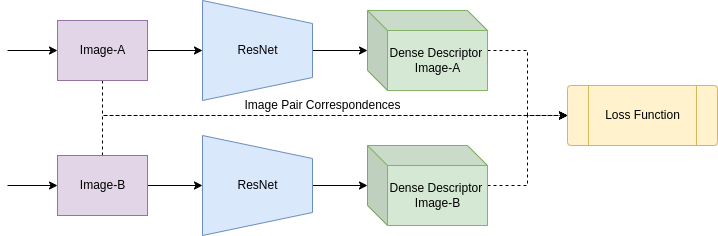
\includegraphics[scale=0.4]{images/don/don_architecture.png}
\end{figure}

\begin{equation}
    \label{eqn:simclr}
    f_{SimCLR}:I \in \mathbb{R}^{H \times W \times 3} \rightarrow x \in \mathbb{R}^D \quad ,\acs{s.t.} \ D \in \mathbb{N}^+.
\end{equation}

\begin{equation}
    \label{eqn:don}
    f_{DON}:I \in \mathbb{R}^{H \times W \times 3} \rightarrow I_D \in \mathbb{R}^{H \times W \times D} \quad ,\acs{s.t.} \ D \in \mathbb{N}^+.
\end{equation}

Furthermore, according to \citeauthor{adrian2022efficient}~\cite{adrian2022efficient}, \ac{DON} relies on sequence of images in the dataset to embed each pixel
to descriptor space by exploiting the geometric prior of objects based on color-hues inturn, generalizing the object.\\

The \ac{ResNet} is usually optimized using mutual image correspondence information of image pairs with contrastive learning on a pixel scale.
The trained network computes a embeddings \ac{s.t.}
the pixel has an unique embedding compared to the rest of the pixels.
The network's visual embedding is invariant to a viewpoint and illumination and comes with the inherent property of generalizing same-class objects.
The visual embedding uniquely describes the pixel locally in an image; hence, referred to as a local descriptor.
The contribution of \ac{DON} is thus its immense ability to generalize for other similar objects within a class without a need to train the network for each such object.



\subsection{Implementation Strategy}

Introduced in 2019, \ac{DON} is young in the research field and applied for use cases in 2021.
In earlier years, the authors of \ac{DON} proposed ``Pixelwise Distribution Loss'' to improve ``Pixelwise Contrastive loss''. This year,
researchers \citeauthor{adrian2022efficient}~\cite{adrian2022efficient} introduced a new loss function called ``Pixelwise NT-Xent Loss'' to make \ac{DON} robust.
The implemented use cases \parencites{rope-manipulation}{block-manipulation}{florence2019self} used different \ac{ResNet} architecture variants
giving an opportunity to test combinations of loss functions with architectures to optimize the network.



\subsection{ResNet Architectures}
\ac{ResNet}-$N$ means that the \ac{DNN} has $N$ convolution layers with shortcuts between them aiding better optimization \cite{resnet}.
E.g., \ac{ResNet}-34 consists of 34 weighted layers. Originally proposed, \ac{ResNet}-34 came with few design rules; to maintain the temporal complexity per layer, the layers had the same number of
filters for the same output feature map size, and the number of filters doubled in that scenario.
The identity shortcuts were employed directly as the input and output dimensions stand the same.\\

With an increase in dimensions, there were two options to consider.
The initial assumption was that the shortcut would continue to conduct identity mapping while padding extra zero entries for expanding dimensions.
The other option was to utilize the projection shortcut to match dimensions.\\

The \ac{ResNet}-50 inherits architecture from the \ac{ResNet}-34 model, with revision in the bottleneck design.
Each of the \ac{ResNet}-34's 2-layer blocks was replaced with a 3-layer bottleneck block, resulting in the deeper \ac{ResNet}-50 design.



\subsection{Loss Functions}


\subsubsection{Pixelwise Contrastive Loss}

The pixelwise constrastive loss is adapted from \cite{simclr} on a pixelwise scale.
The pixelwise contrastive loss brought in the concept of \ac{DON} itself introduced by \citeauthor{florence2018dense}~\cite{florence2018dense}.
The pixelwise constrastive loss function aims
to minimize the distance between the embeddings corresponding to a match, while the embeddings corresponding to
a non-match are set at least by a marginal distance $M$ apart. The loss function is described as,

\begin{equation}
    \mathcal{L}_{matches} = \dfrac{1}{N_{matches}} \displaystyle\sum^{N}_{i, j} \left\Vert f(I_a)[x_i, y_j] - f(I_b)[x_i, y_j] \right\Vert,
\end{equation}

\begin{equation}
    \mathcal{L}_{non-matches} = \dfrac{1}{N_{non-matches}} \displaystyle\sum^{N}_{i, j} max(0, \ M - \left\Vert f(I_a)[x_i, y_j] - f(I_b)[x_i, y_j] \right\Vert),
\end{equation}

\begin{equation}
    \mathcal{L}_{Total} = \mathcal{L}_{matches} + \mathcal{L}_{non-matches}.
\end{equation}

$M$ is a hyperparameter and has to be chosen optimally while training the network.
The loss function is sensitive to batch size and number of correspondences \parencites{adrian2022efficient}{florence2020dense}.
Additionally, non-matching correspondences needs to be sampled for training the network.
This thesis is not going to benchmark this loss function as it is outdated and comes with drawbacks compared to newly proposed loss functions.


\subsubsection{Pixelwise Distribution Loss}

Introduced in \citeauthor{florence2018dense}~\cite{florence2018dense}, the pixelwise distribution loss function aims to compute a set of probability distributions for each keypoint $k = \{1, 2, \ldots K\}$
minimizing the divergence between the predicted heatmap and the ground truth heatmap described as,

\begin{equation}
    \label{eqn:spat_exp}
    p_a(x_i, y_i | f(I_a), f(I_b), x_b, y_b) = \dfrac{K(f(I_b)[x_b, y_b], f(I_a)[x_i, y_j])}{\displaystyle\sum_{i', j'}K(f(I_b)[x_b, y_b], f(I_a)[x_i', y_j'])},
\end{equation}

\noindent where, the $K:(\mathbb{R}^{\mathbb{N}^+}, \mathbb{R}^{\mathbb{N}^+}) \rightarrow \mathbb{R}$ is a kernel function and
it can be of any formulation as long as it yields a scalar ($\mathbb{R}$) processing two vectors of the same dimension.
The term, $p_a(x_i, y_i | f(I_a), f(I_b), x_b, y_b) \in [0, 1]$ is the spatial probability of a keypoint in $f(I_a)[x_a, y_a]$ in the image $f(I_b)$.\\

The spatial expectation from the spatial probability is computed as,

\begin{equation}
    \label{eqn:x_exp}
    \hat{x_b} = \displaystyle\sum_i^W p_a(x_i | f(I_a), f(I_b), x_b) x_i,
\end{equation}

\begin{equation}
    \label{eqn:y_exp}
    \hat{y_b} = \displaystyle\sum_i^H p_a(y_i| f(I_a), f(I_b), y_b) y_i,
\end{equation}

The spatial loss of $I_a[x_a, y_a]$ in $I_b[x_b, y_b]$ is computed as,

\begin{equation}
    \mathcal{L}_{b \rightarrow a} = \| x_b - \hat{x_b} \| + \| y_b - \hat{y_b} \|,
\end{equation}

The total bi-directional loss is computed as,
\begin{equation}
    \mathcal{L}_{Total} = \mathcal{L}_{b \rightarrow a} + \mathcal{L}_{a \rightarrow b},
\end{equation}

The kernel functional chosen to compute the bi-directional loss function,
\begin{equation}
    K: (f(I_a)[x_i, y_i], f(I_b)[x_b, y_b]) \rightarrow exp(-\|f(I_a)[x_i, y_i] - f(I_b)[x_b, y_b] \|).
\end{equation}

\begin{figure}[htb]
    \centering
    \captionsource{2D spatial expectation of keypoint in two images.}{\cite{florence2020dense}}
    \label{fig:spat_exp}
    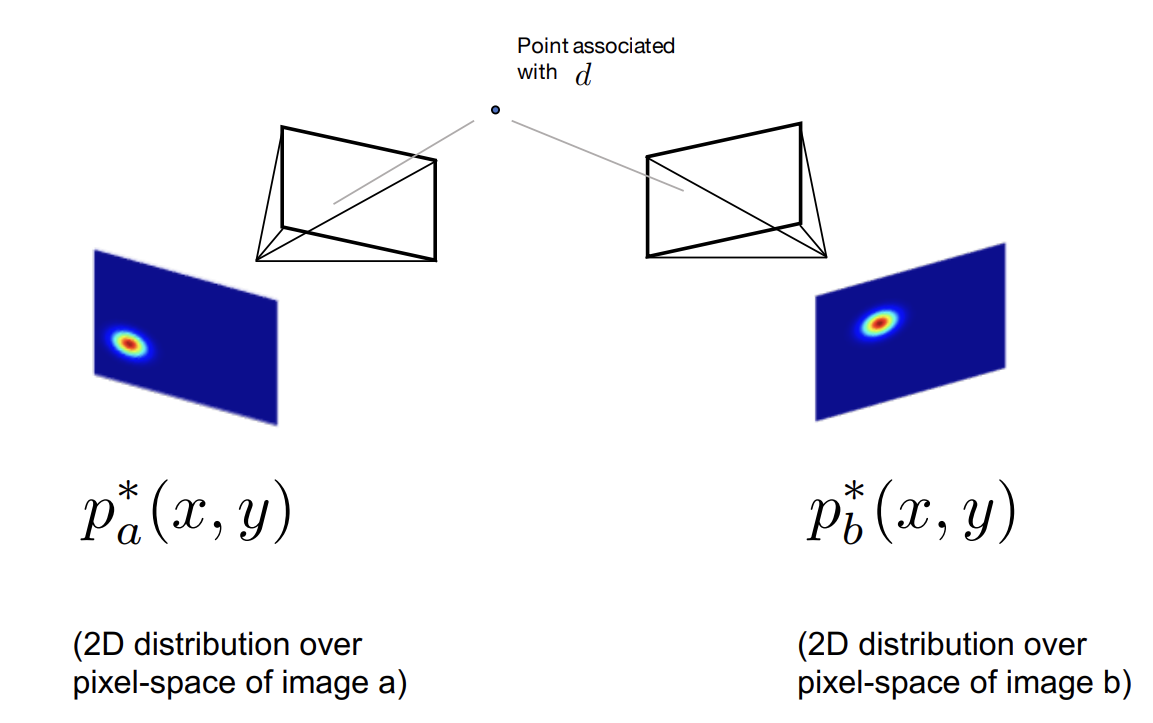
\includegraphics[scale=0.17]{images/spatial_expectation.png}
\end{figure}

This pixelwise distribution loss function can be implemented in a batch fashion yielding high-performance computation time in a computer.
Furthermore, The Figure~\ref{fig:spat_exp} intuitively illustrates the spatial expectation of a keypoint in two images.\\

Furthermore, the loss function improves spatial expectation of a descriptor compared to the pixelwise contrastive loss,
yielding better results in the search space of a descriptor in a new image.
One of the drawbacks of using this loss function is that only one object belonging to the same class in an image can
be used while training the neural network. Having more objects belonging to the same class yields faulty prediction of spatial expectations.

\subsubsection{Pixelwise NT-Xent Loss}

The ``NT-Xent loss'' is originally introduced in \citeauthor{simclr}~\cite{simclr} adopted by \citeauthor{infonce}~\cite{infonce} to encode an entire image to an embedding and implemented on a pixel level
to train \ac{DON} by \citeauthor{adrian2022efficient}~\cite{adrian2022efficient}. The authors \citeauthor{adrian2022efficient}~\cite{adrian2022efficient} randomly sample $N$ correspondences from an
image pair $(I_A, I_B)$, with each correspondence yielding two descriptors $d^A_i$ and $d^B_i$ , for a total of $N$ pairs, or
$2N$ descriptors. For a given descriptor, all other $2(N - 1)$ descriptors are respectively treated as negative examples.
The below given loss function is directly optimized against the descriptor pair,

\begin{equation}
    \mathcal{L}_{i, j} = -\log \dfrac{\exp(K(d_i, d_j) / \tau)}{\sum^{2N}_{k=1, k \neq i} \exp(K(d_i, d_j) / \tau)},
\end{equation}

where, $\tau \in \mathbb{R}^+$ is a temperature scaling factor and $K$ is cosine similarity kernel defined as,

\begin{equation}
    \label{eqn:cosine_similarity}
    K = \dfrac{\left< d_i, d_j \right>}{\| d_i\| \| d_j\|} \quad ,\ac{s.t.} \ d_{i, j} \in \mathbb{R}^{\mathbb{N}^+}, \ K \in  [1, 0].
\end{equation}

Since $K$ takes only positive inputs, unlike the cosine function, it produces the outputs in the range [0, 1] which leads to its interpretation as in expression refer equation \ref{eqn:kernel}.

\begin{equation}
    \label{eqn:kernel}
    K(d_i, d_j) = \begin{cases}
        1 & \implies (d_i, d_j) \text{ are similar}.    \\
        0 & \implies (d_i, d_j) \text{ are dissimilar}.
    \end{cases}
\end{equation}

One of the drawbacks of the pixelwise nt-xent loss function is that semantically closer objects in an image are treated as two different objects which in turn
hinders the generalizing properties of the neural networks.

\subsection{$PCK@k$ as an Evaluation Metric}

To measure the performance of the network, ``$PCK@k$'' evaluation metric is adopted as in preceding works \parencites{pck}{adrian2022efficient}. $PCK@k$ is defined
for a set of pixel pairs $\mathcal{T} = \{p_i, q_i \}^N_{i=1}$ as follows,

\begin{equation}
    \label{eqn:pck}
    PCK@k(\mathcal{T}) = \dfrac{1}{|\mathcal{T}|} \displaystyle\sum_{(p_i, q_i) \in \mathcal{T}} [ \|p_i - q_i\| \leq k] \quad ,\ac{s.t.} \ (p_i, q_i) \in \mathbb{R}^{\mathbb{N}^+}, (k, \mathcal{T}) \in \mathbb{R},
\end{equation}

\noindent where $k$ is the maximum error allowed in turn, influencing the Iverson bracket $[ \ \cdot \ ]$  to 1 if the error is within the limits of $k$ and 0 otherwise.
$\mathcal{T}$ is a number of keypoints ($p_i, q_i$) normalizing the computed metric. Instead of using $L^2$-Norm to compute the error between keypoints, it
is replaced by a kernel function `$D$' similarly in equation~\ref{eqn:cosine_similarity} in page~\pageref{eqn:cosine_similarity} bringing in more flexibility.
The kernel revised metric is described as,

\begin{equation}
    PCK@k(\mathcal{T}) = \dfrac{1}{|\mathcal{T}|} \displaystyle\sum_{(p_i, q_i) \in \mathcal{T}} D(p_i, q_i) \leq k.
\end{equation}


\subsection{Suzanne, a synthetic dataset}

To train and benchmark \ac{DON}, no compatible ready datasets are available. The datasets available either missed camera information like intrinsics or extrinsics parameters,
masks information or captured same objects belonging to the same
class in an image, posing ill-conditions to benchmark pixelwise distribution loss.\\

To overcome this situtation, `BlenderProc'~\cite{blenderproc} is used to generate synthetic dataset with all annotations needed to train \ac{DON}.
`Suzanne' is a model already available in the render tool and is
placed in the world datum center. For this control dataset, 100 random cameras are added in the environment with random poses capturing depth,
extrinsic information and mask for each viewpoint. The Table~\ref{table:suzanne} in page~\pageref{table:suzanne},
provides the preview of dataset. The annotated pixels in blue in second image from right to left in Table~\ref{table:suzanne} projects the correspondences through world
coordinates in the first image from right to left annotated in red. As the dataset produces perfect depth maps of the objects in the images,
the benchmarking metrics might not tally with available benchmarked results.\\


\begin{table}[htb]
    \centering
    \begin{tabular}{ccccc}
        \hline
        \multicolumn{5}{c}{Dataset Preview}                                                                                                                                                                                                                                                                                                                                                               \\ \hline
        \multicolumn{1}{c}{RGB}                                                    & \multicolumn{1}{c}{Depth}                                                 & \multicolumn{1}{c|}{Mask}                                                    & \multicolumn{2}{c}{Correspondences Mapping}                                                                                                               \\
        \multicolumn{1}{c}{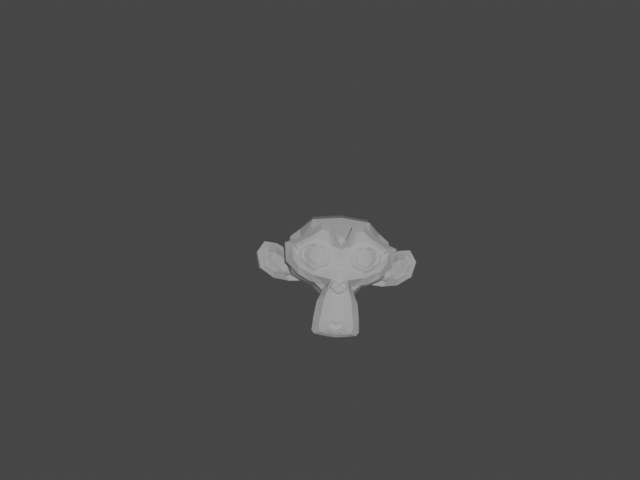
\includegraphics[scale=0.12]{images/suzanne/9_rgb.png}} & \multicolumn{1}{c}{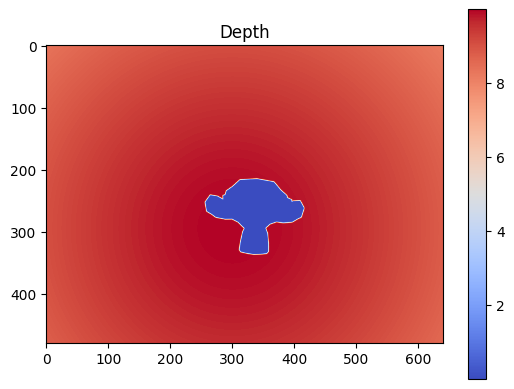
\includegraphics[scale=0.2]{images/suzanne/depth.png}} & \multicolumn{1}{c|}{
\includegraphics[scale=0.12]{images/suzanne/9_mask.png}} & \multicolumn{1}{c}{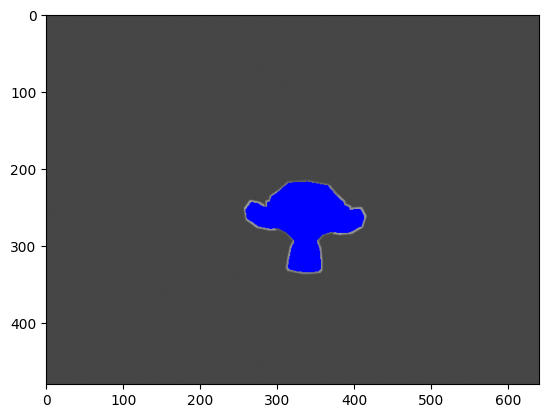
\includegraphics[scale=0.2]{images/suzanne/output.png}} & \multicolumn{1}{c}{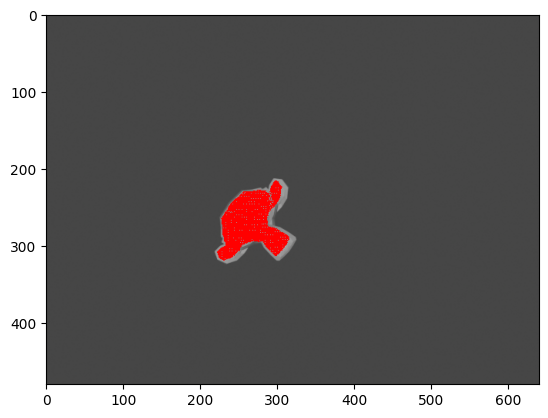
\includegraphics[scale=0.2]{images/suzanne/output_1.png}} \\ \hline
    \end{tabular}
    \caption{Depiction of dataset quintennsials features of dataset}
    \label{table:suzanne}
\end{table}



Following the procedure in \cite{hartley2003multiple}, the correspondences are computed in an image pair described as follows:

\noindent The camera extrinsic parameters ($\mathcal{T}_{C \rightarrow W} \in \mathbb{R}^{4 \times 4}$) is the camera pose relative to the world frame.
The camera intrinsics is defined as $\mathcal{I} \in  \mathbb{R}^{3 \times 3}$.
To map the correspondences from image $I_a$ to image $I_b$, the pixels from the image $[u,v]^T \in I_a \in \mathbb{R}^{2 \times 1}$
are projected to the world coordinates $W_a \in \mathbb{R}^{3 \times 1}$ using depth ($d$) and from the world coordinates to the image $I_b$ as follows:

\begin{equation}
    \label{eqn:world_proj}
    W_a = \mathcal{T}_{C \rightarrow W}^a \ \mathcal{I}^{-a} \ \begin{bmatrix}
        u^a \\
        v^a \\
    \end{bmatrix} \ d_{uv}^a
\end{equation}

The computed world coordinates from $I_a$, $W_a$ are projected to pixels in $I_b$,

\begin{equation}
    d_{uv}^b \ \begin{bmatrix}
        u^b \\
        v^b \\
    \end{bmatrix} =  \mathcal{I}^b \ \mathcal{T}_{C \rightarrow W}^{-b} \ W_a,
\end{equation}

\noindent where,
\begin{equation}
    \mathcal{T}_{C \rightarrow W}^{-b} = \begin{bmatrix}
        R^b   & -R^b t^b \\
        0^T_3 & 1
    \end{bmatrix}, \quad \ac{s.t.} \ R^b \in SO(3).
\end{equation}

Additionally, mask is used to sample the pixels from $I_a$ within the object silhouette.



\subsection{Manual Method for Robot Grasp Generation}

The \ac{DON} produces visual embeddings ($f(I)[u, v] \rightarrow d, \quad d \in \ \mathbb{R}^{\mathbb{N}+}$) such that each pixels withholds unique embedding in descriptor space
reducing computational complexity to find the same pixel in different viewpoint in an \ac{RGB} space omitting complex search algorithm. Using ``Pygame'' \cite{pygame} library in python, an interactive
application is developed to pick descriptors in the descriptor space with it's image coordinates {$[u, v]^T$} using depth and camera intrinsics to project them to the coordinates in the camera frame. More than
three descriptors are picked such that it produces a valid rotation matrix via \ac{PCA} or \ac{SVD} and the mean value acting as a center to generate a 6D pose defined as,

\begin{equation}
    \mathcal{T} = \begin{bmatrix}
        R     & t \\
        0^T_3 & 1
    \end{bmatrix} \in \mathbb{R}^{4 \times 4}, \quad \ac{s.t.} \ R \in SO(3), \ t \in \mathbb{R}^{3 \times 1},
\end{equation}

The interactive application allows to save multiple object pose definition file and this definition file is loaded into an other application to search and compute multiple object
6D pose information in an other or same image. The descriptors are searched using gaussian kernel derived from heat kernel formulation,

\begin{equation}
    \label{eqn:gaussian_kernel}
    \mathbb{E}{[u^*, v^*]_{d}} = \operatorname*{argmin}_{u_i, v_i} \ exp-\left(\dfrac{\|(f(I_a)[u_i, v_i] - d)\|}{exp(t)}\right)^2
\end{equation}

Where $t \in \mathbb{R}$ controls the kernel width influencing the search space to compute the spatial expectation of the query descriptor $d$ in image $I_a$.
The descriptors produced by \ac{DON} are supposedly to be robust against color jitters, illumination changes and occlusions in order to produce consistent 6D poses \cite{adrian2022efficient}.\\

To compute the relative 6D pose of an object in the new viewpoint of the camera, the queried keypoint locations are redordered in the matrix respective to the keypoint
and its spatial locations as stored in the definition file.
If a keypoint is not found, then the keypoint in the definition file is omitted and mutually rearranged. The queried keypoint locations produce relative 6D pose $\mathcal{T}_{object}$
compared to the pose stored in the definition file as,

\begin{equation}
    \mathcal{T}_{rel} = (\mathcal{T}_{def}^T \ \mathcal{T}_{def})^{-1} \ \mathcal{T}_{def}^T \ \mathcal{T}_{object}.
\end{equation}

To eliminate the manual process of annotating keypoints to genetate robot grasps, KeypoinNet is implemented.


\section{KeypointNet}

KeypointNet is a framework for end-to-end geometric reasoning that regresses the best set of category-specific 3D keypoints with their associated detectors, i.e., higher-dimensional generalized embeddings.
By definition, KeypointNet works for an image pair.
This framework estimates 3D pose by giving a differentiable goal that seeks the optimal set of keypoints to recover the relative pose of an item between two viewpoints.
Hence, KeypointNet allows for predicting geometrically and semantically consistent keypoints across viewing angles and instances of an object category by optimizing four loss functions.\\


\subsection{Loss functions}

The KeypointNet produces $N$ number of spatial probabilities for $N$ keypoints described by $g_i(u,v) \in \mathbb{R}^{W \times H}, \ac{s.t.} \ \sum_{u,v} g(u,v) = 1$.
The pixel spatial expectations is computed via continuous sampling method described by,

\begin{equation}
    [u_i, v_i]^T =  \left[ \displaystyle\sum_{u, v} g_i(u, v) * u , \  \displaystyle\sum_{u, v} g_i(u, v) * v \right]^T, \quad \ac{s.t.} \ g_i(u,v) \in \mathbb{R}^{W \times H}.
\end{equation}

\noindent Similarly, depth is computed as follows:
\begin{equation}
    d_i = \displaystyle\sum_{u, v} g_i(u, v) * d_i[u, v], \quad \ac{s.t.} \ d_i(u,v) \in \mathbb{R}^{W \times H}.
\end{equation}

The self-supervised training of this network is based on the following loss functions.






\subsubsection{Multiview Consistency Loss}

The multiview consistency loss function enforces the network to regress keypoint expectations at same the locations in an image pair.
Concisely, a keypoint in one image should project on a pixel location corresponding to a keypoint in another image.
To achieve this, pixels are projected to the camera frame using depth and intrinsic information. Using mutual transformation information
between two cameras, the pixels are further projected back to the pixel frame of the second camera. The loss is then the distance between the projected pixel location and
regressed keypoint's pixel location. \\

To make this formulation more intuitive, the originally proposed method is altered. Instead, of evaluating the keypoints in pixel frame, they are evaluated in the world frame.
The idealogy is that the object is fixed in the world datum and camera poses changes preserving the object coordinates in the world frame as depicted in Figure~\ref{fig:spat_exp} in page~\pageref{fig:spat_exp}.
The altered multiview consistency loss function is defined as,

\begin{equation}
    \mathcal{L}_{mvc} = \dfrac{1}{N} \displaystyle\sum^N_{i=1} \| W_A^i - W_B^i\|, \quad \ac{s.t.} \ W_{A, B} \in \mathbb{R}^{3 \times 1}.
\end{equation}





\subsubsection{Relative Pose Loss}

As the KeypoinNet produces $N$ number of keypoints, the keypoint locations together projected into the camera frame coordinates produces a 6D pose computed.
The relative pose loss function rearranges the keypoint locations in an image preserving the object's 6D pose in the viewpoint respective to the camera pose.
Additionally, this preserves the relative pose between two camera poses and relative pose generated from the keypoint locations in an image pair.\\

As per the original implementation of the KeypointNet, the authors discard the relative translation and expressed the relative pose
loss in form of chordal distance between two rotational matrices $ \in SO(3)$ using Frobenius-Norm \cite{bhatia2013matrix} as:

\begin{equation}
    \mathcal{L}_{pose} = 2 \arcsin \left( \dfrac{1}{2\sqrt{2}} \left\Vert \hat{R} - R \right\Vert_F \right) \quad,\ac{s.t.} \ R \in SO(3).
\end{equation}

Where, $\hat{R}$ is the groundtruth relative rotation of camera-a pose in the world frame and camera-b pose in the world frame and $R$ is the predicted relative rotation of regressed keypoints in an image pair.
The Frobenius norm yields the chordal distance in range $[0, 2 \sqrt{2}]$ which is normalized in the implementation.
The chordal distance formulation satisfying the triangle inequality condition involves ``\emph{some messy algebra}'' \cite{huynh2009metrics} as the operation $\hat{R} - R \notin SO(3)$. \\


To make this more geometrically intuitive, the poses $\in SE(3)$ are transported to $Riemannian$ $manifold$ \cite{lee2018introduction}.
$Riemannian$ $manifold$ is rich in geometry and differentiably smooth.
Instead, of expressing the distance in chordal form, `geodesic-distance' is chosen as it is smooth on for infinitesimally small trajectories on the manifold.
Here, the trajectory is defined as the distance to be covered such that the two rotation matrices align with each other.\\

The manifold geometry consists of two parts, i.e., a manifold and  a tangential plane tangential place $T(\mathcal{M}^p)$ represented as a tangential Euclidean space to the manifold, and the manifold space. the manifold space \( \mathcal{M}^p: p \in \mathbb{R}^{N^+}\).
Exp-maps and log-maps refer equation~\ref{eqn:logmap} are used to transport a vector on tangential plane to the manifold and vice versa.

\begin{equation}
    expmap: \mathfrak{so}(3) \rightarrow SO(3),
\end{equation}

\begin{equation}
    \label{eqn:logmap}
    logmap: SO (3) \rightarrow \mathfrak{so}(3).
\end{equation}

Here $r(\alpha) \in \mathfrak{so}(3) \in  T(\mathcal{M}^p)$ is a skew-symmetric matrix built from the axis angles $\alpha \in \mathbb{R}^3$ described as,

\begin{equation}
    r(\alpha) = \begin{bmatrix}
        0  & -z & y  \\
        z  & 0  & -x \\
        -y & x  & 0
    \end{bmatrix} \quad, \ac{s.t.} \ \alpha = [x, y, z]^T \in  \mathbb{R}^3.
\end{equation}

The object or camera's rotation in the dataset is represented as $SO(3)$.\\

The geodesic distance is a \emph{bi-invariant} metric on $SO(3)$ with range[0, $\pi$]:
\begin{equation}
    \label{eqn:geodesic}
    \mathcal{L}_{pose} = \dfrac{1}{\sqrt{2}} \| logmap(\hat{R}^T R) \|_F = \dfrac{1}{2} \| logmap(\hat{R}^T R) \|.
\end{equation}

The $\mathcal{L}_{pose}$ is substituted in the place of original loss function formulation.
The relative groundtruth rotation ($\hat{R}$) for the loss is computed as:

\begin{equation}
    \hat{R} = \hat{R}_{A \rightarrow B} = \hat{R}_A^{T} \ \hat{R}_B \quad,\ac{s.t.} \ \hat{R} \in SO(3).
\end{equation}

\noindent where, $\hat{R} = \hat{R}_{A \rightarrow B} \in \mathbb{R}^{3 \times 3}$ is the groundtruth relative rotation of camera-a pose in world $\hat{R}_A$ and camera-b pose in the world $\hat{R}_B$.
The camera poses are the extrinsic matrices available in the dataset. To compute the relative rotation $R$ of regressed keypoints
in an image pair, i.e., $X_A, X_B \in \mathbb{R}^{N \times 3}$ Kabsch's algorithm \cite{kabsch} is employed as follows:

\begin{equation}
    \mathcal{H} = (X_A - X_A^{mean})^T \ (X_B - X_B^{mean}) \quad,\ac{s.t.} \ \mathcal{H} \in \mathbb{R}^{3 \times 3}, \ X^{mean}_{A,B} = \overline{X}_{A,B}.
\end{equation}

\noindent where, $\mathcal{H}$ is the covariance matrix of the mean centered keypoint locations in the camera frame. To center the keypoint locations in the camera frame,
$X^{mean} \in \mathbb{R}^{1 \times 3}$ is computed along the dimension $N$ and each row in $X$ is subtracted with the mean.
The predicted relative rotation of keypoint locations in the image pair is computed as,

\begin{equation}
    R_B = V \begin{bmatrix}
        1 & 0 & 0          \\
        0 & 1 & 0          \\
        0 & 0 & det(V U^T)
    \end{bmatrix} U^T,
\end{equation}

where,

\begin{equation}
    U \Sigma V^T = SVD(\mathcal{H}).
\end{equation}

The term $det(V U^T)$ handles the reflection case while estimating the rotation matrix. In other terms it makes the $z$ rotation vector orthonormal to `$xy$'
rotation vectors such that it always points to the camera in the camera relative frame. This method to condition $z$ rotation vector produces gradients which allows neural networks
to be trained via backpropogation compared to using cross-product of vectors which does not produce gradients since the vector in the matrix is changed via inplace operation.









\subsubsection{Separation Loss}

Separation loss function penalizes cases where the distance between two keypoint locations is less than a specified margin ($\delta$).

\begin{equation}
    \mathcal{L}_{sep} = \dfrac{1}{N} \displaystyle\sum_i^N \displaystyle\sum_{j\neq i}^N max(0, \delta^2 - \| X_i - X_j \|^2).
\end{equation}







\subsubsection{Silhoutte Loss}

Silhoutte loss functions encourages the spatial probabilities of keypoints $g_i(u, v)$ to lie with the object silhoutte:

\begin{equation}
    \mathcal{L}_{obj} = \dfrac{1}{N} \displaystyle\sum^N_{i=1} -log \displaystyle\sum_{u, v} b[u, v] \ g_i(u, v).
\end{equation}

While training the network, the mask of the object is accessible. The mask values are sampled from the pixel locations $b[u, v] \in \{0, 1\}$. The mask information is only used
while training the network and is not using during the inference. If all the keypoints are regressed within the object silhoutte, the loss computes to zero.








\subsubsection{Variance Loss}

Variance loss function penalizes the spatial probabilities if they are broad in turn, encouraging peaky distribution.
The broader spatial probabilities brings in more uncertainty in the keypoint spatial expectation.
In turn, the loss function penalizes the uncertainty of the keypoint spatial expectation by shrinking the span of the spatial probabilities as depicted in Figure~\ref{fig:var_loss} in page~\pageref{fig:var_loss}.
Furthermore, in the Figure~\ref{fig:var_loss} in page~\pageref{fig:var_loss}, the x marks the keypoint spatial expectation. The left image illustrates the broader spatial probability of a keypoint bringing in more
uncertainty in the keypoint spatial location (expectation). The right image describes the peaky spatial probability of the keypoint encouraged by the loss function. \\

The variance loss functions is described as,

\begin{equation}
    \mathcal{L}_{var} = \dfrac{1}{N} \displaystyle\sum^N_{i=1} \displaystyle\sum_{u, v} g_i(u, v) \left\Vert \mathcal{G} - [u_i, v_i]^T \right\Vert^2,
\end{equation}

where $\mathcal{G}$ is the spatial grid of row and column indices described as,

\begin{equation}
    \label{eqn:spatial_grid}
    \mathcal{G}_{0ij} = \begin{bmatrix}
        0      & \dots  & 0      \\
        \vdots & \ddots & \vdots \\
        H      & \dots  & H
    \end{bmatrix}, \quad
    \mathcal{G}_{1ij} = \begin{bmatrix}
        0      & \dots  & W      \\
        \vdots & \ddots & \vdots \\
        0      & \dots  & W
    \end{bmatrix} \quad \quad,\ac{s.t.} \ \mathcal{G}  \in \mathbb{R}^{2 \times W \times H}.
\end{equation}

\begin{figure}[htb]
    \centering
    \caption{Variance loss function at work.}
    \label{fig:var_loss}
    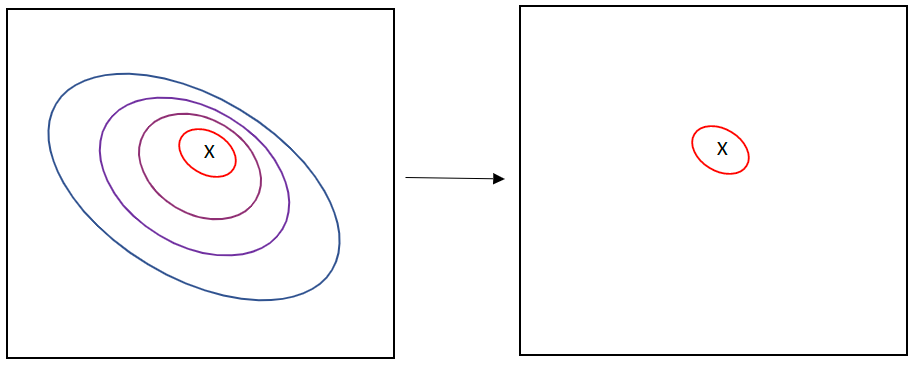
\includegraphics[scale=0.15]{images/keypointnet/var_loss.png}
\end{figure}

\subsection{Total Weighted-Sum Loss}

To train the network, all loss functions are weighed by their own specific weights inturn, signifying that one loss functions needs more priority than other loss functions.
The priority depends on the network architecture being used. Let's say if the multiview consistency loss is not converging, then the weights assigned to that particular loss function
are increased such that the multiview loss is further optimized by the network in the training phase. The total weighted loss function is the scalar product of the weights $W = [w_{mvc}, w_{pose}, w_{sep}, w_{obj}, w_{var}]^T $ and the individual
loss functions $ \mathcal{L} = [\mathcal{L}_{mvc}, \mathcal{L}_{pose}, \mathcal{L}_{sep}, \mathcal{L}_{obj}, \mathcal{L}_{var}]^T$ described as,

\begin{equation}
    \label{eqn: weighted_sum}
    \mathcal{L}_{Total} = < W, L > \quad,\ac{s.t.} \ \mathcal{L}_{Total} \in \mathbb{R} \ \& \ W,L \in \mathbb{R}^4.
\end{equation}

Here $W$ is a hyperparameter. The hyperparameter in this thesis implementation will be fixed by a trial-and-error process as other sampling or optimization process consumes a lot of time.

\subsection{Network Modification}

The \ac{ResNet} architecture will be used over originally proposed image segmentation based \ac{CNN} while preserving the part of architecture with
predicting depth and spatial probabilities of the keypoints to preserve the neural network architecture homogenity with \ac{DON} architecture.\\

Additionally, no pretrained orientation network is used to aid the KeypointNet breaking the symmetry of the objects as in \cite{suwajanakorn2018discovery}.
As per the proposed data augmentation in \cite{suwajanakorn2018discovery}, the data will not be scaled to a unit dimension preserving realistic
conditions of object in an environment for which the network will be trained for.





\section{End-to-End Network Training}

\emph{End-to-end network training} is a deep learning technique in which all parameters are taught concurrently rather than step by step.
An deep learning method is trained in an end-to-end manner when a \ac{DNN} needs to perform multiple tasks. Furthermore, sometimes a deep learning network learns
joint features pertaining multiple tasks. Particularly in this thesis, joint features for \ac{DON} representations and generalized object 6D poses are
computed via generalized geometrically consistent keypoints.\\




\subsection{KeypointNet Informed Dense Object Nets}

The depth values produced for small \& shiny objects by the consumer grade depth cameras are not accurate \cite{kupcsik2021supervised}, in turn
leading to inconsistent correspondences mapping between two image pairs which further leads to inaccurate training of \ac{DON}. To overcome this, KeypointNet is employed as KeypointNet
does not depend on the depth values of objects for training. \\

As per the definition, KeypointNet can be modified to generate correspondences between image pair
belonging to the same class without the need of additional \ac{DNN} like Universal Correspondence Network \cite{ucn}. KeypointNet eliminates the need for projecting
pixels from one image to another image through the world coordinates Equation \ref{eqn:world_proj} in page \pageref{eqn:world_proj} to compute correspondences in an image pair.\\

Furthermore, the KeypointNet architecture is stacked on top of \ac{DON} architecture such that semantic correspondences are supplied for \ac{DON} seamlessly keeping it self-supervised.
Both the networks are optimized with the joint losses and not individually as described below:


\begin{equation}
    \label{eqn:joint_loss}
    \mathcal{L}_{Joint} = \mathcal{L}_{KeypointNet} + \mathcal{L}_{DON}
\end{equation}

The joint losses produces mutual gradients for optimization such that the networks compute features which are beneficial to each other forming a coordination
to fulfil a task \cite{levine2016end}.\\

Furthermore, \ac{DON} training is delayed by few epochs and the KeypointNet is trained at the start such that the training converges faster.


\subsection{Dense Object Nets Informed KeypointNet}
\label{section: DON-KeypointNet}

Preserving the goal of the thesis, single class generalized labels need to be stored for deployment and to achieve this, \ac{DON} is stacked on top of KeypointNet.
As \ac{DON} produces class generalized descriptors (labels) the KeypointNet is employed to pick the labels autonomously.\\

The KeypointNet regresses $N$ number of keypoints in the descriptor image and each keypoint is a pixel location for the label in the descriptor image.
For an object, class generalized keypoints are stored in $N$ random probabilities. This insures that in cases of object occlusion in viewpoint, if one label is not found, another label can be recalled
creating a grasping point for the robot as a counter-measure.\\

For better optimization, the \ac{DON} is trained first and few epochs later KeypointNet is optimized better.
Additionally, the joint losses is adopted as in Equation \ref{eqn:joint_loss} in page \pageref{eqn:joint_loss} for optimization purposes.




\subsection{Mining Dense Object Nets Representations in KeypointNet}

The KeypointNet predicts semantic object keypoints, in turn equipping inert property for object generalization. \ac{DON} computes dense
generealized visual embeddings by exploiting the geometric prior of a sequence of registered RGBD frames to sample pixel correspondences
between alternative views of the same object based on color hues \cite{adrian2022efficient}.\\

The KeypointNet shares the same \ac{ResNet} architecture as \ac{DON} ushering an idea that the KeypointNet might be encompassing generalized
visual embeddings similarly computed by \ac{DON}.
Intuitively, upsampled dense ouput features as depicted in the Figure~\ref{fig:keynet} from the \ac{ResNet} architecture in the KeypointNet might have the dense object representations.\\

The KeypointNet is trained with the upsampled dense feature having output channel dimension of 256 and for
benchmarking purposes, it is set to $D=16$ such that it can be mutually benchmarked against \ac{DON} computed representations.\\

The key adavantage here is that the dense object representations can be directly extracted by upsampling the output of the last
layer without the need of training \ac{DON} saving time and resources. The same procedure is employed to store prioritized labels as
in section \ref{section: DON-KeypointNet} in page \pageref{section: DON-KeypointNet}.


\begin{figure}[htb]
    \centering
    \caption{KeypointNet Architecture.}
    \label{fig:keynet}
    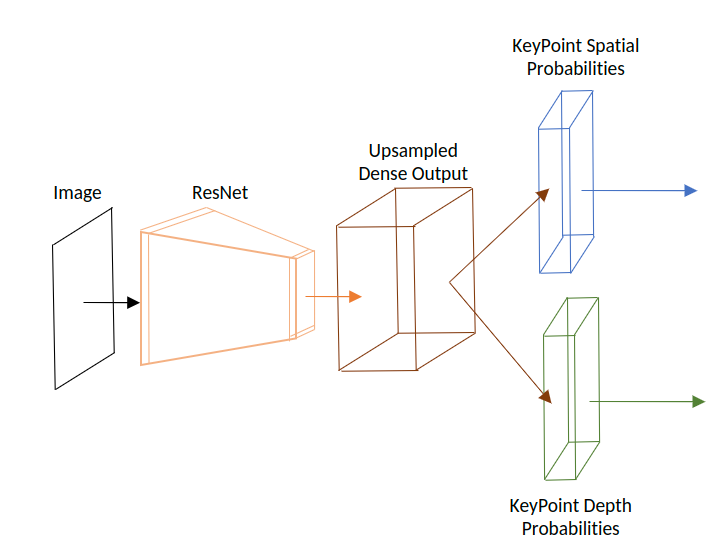
\includegraphics[scale=0.3]{images/keypointnet/arch.png}
\end{figure}

\section{Generalizing ``Caps''}

The thesis moreover chooses to generalize caps. We have chosen the cap object for the further examination since the cap mesh models are readily available in the Shapenet library~\cite{chang2015shapenet}
and it was also possible to obtain the real-world cap data. Blenderproc~\cite{blenderproc} is used to generate the synthetic cap dataset similar to Suzanne dataset.
Caps are chosen such that each of them have distinct shapes, designs and colors. The cap models are chosen from the Shapenet library~\cite{chang2015shapenet} library
as it possess rich object information including textures, as one can see in Table~\ref{table:cap_dataset} in page~\pageref{table:cap_dataset}.\\

\begin{table}[htb]
    \centering
    \begin{tabular}{ccccc}
        \hline
        \multicolumn{5}{c}{Cap Dataset Preview}                                                                                                                                                                                                                                                                                                                \\
        \multicolumn{1}{c}{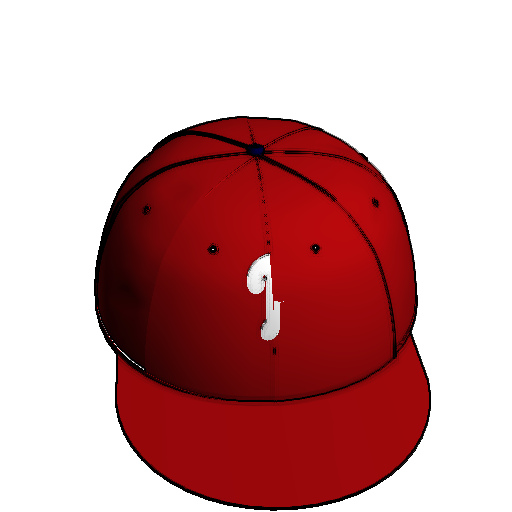
\includegraphics[scale=0.12]{images/cap/1.png}} & \multicolumn{1}{c}{
\includegraphics[scale=0.12]{images/cap/2.png}} & \multicolumn{1}{c}{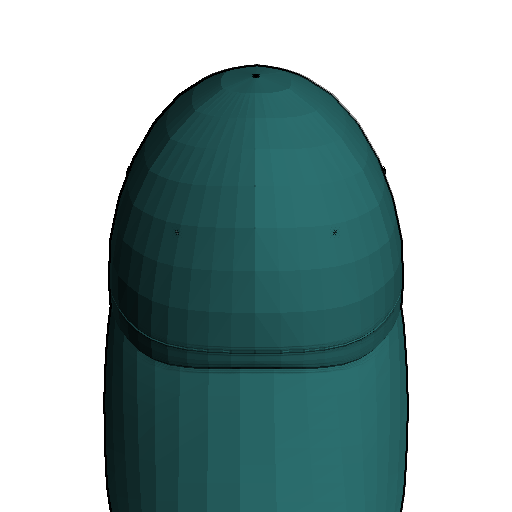
\includegraphics[scale=0.12]{images/cap/3.png}} & \multicolumn{1}{c}{
\includegraphics[scale=0.12]{images/cap/4.png}} & \multicolumn{1}{c}{
\includegraphics[scale=0.12]{images/cap/5.png}} \\ \hline
    \end{tabular}
    \caption{Illustration of caps sampled from the Shapenet library~\cite{chang2015shapenet}.}
    \label{table:cap_dataset}
\end{table}

To make the training more robust such that networks are more object-centric, the images are additionally augmented with random backgrounds and noisy backgrounds in
addition to color jitter and greyscaling augmentations, as depicted in Figure~\ref{fog:back_augmentations} in page~\pageref{fog:back_augmentations}. The mask information in the synthetic dataset is used to augment the backgrounds.

\begin{figure}[htb]
    \centering
    \caption{The image in the right illustrates the noisy backgrounds and the image in left describes random background augmentation.}
    \label{fog:back_augmentations}
    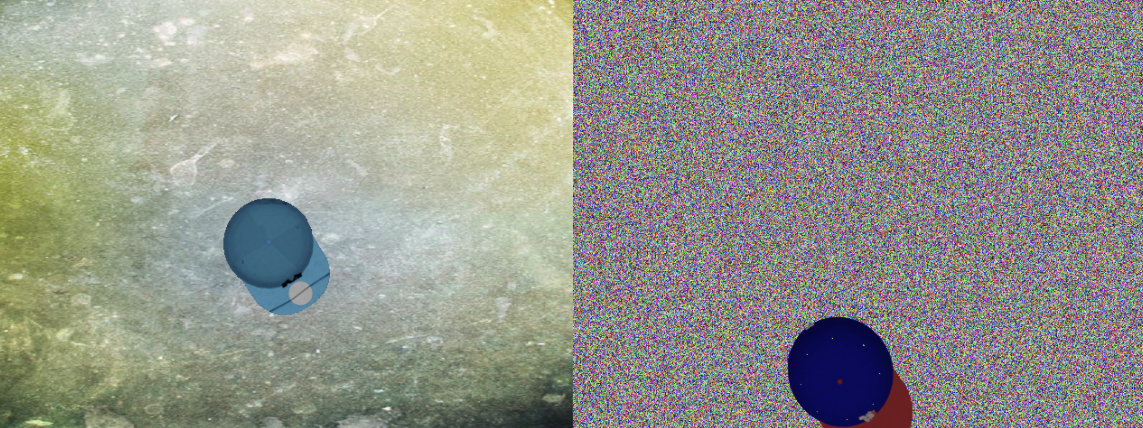
\includegraphics[scale=0.2]{images/cap/back_augs.png}
\end{figure}


\subsection{Semantic Correspondences Mapping Pipeline}

By definition, KeypointNet regresses semantic keypoints on the objects. Meaning, the keypoint in one object is positioned semantically equivalent in an another object of the same class.\\

Furthermore, this property of KeypointNet of producing semantic keypoints in the inference stage and not training phase can be used as correspondences in an image pairs to train \ac{DON}.
Loading semantic equivalent correspondences might affect the evalutaion of \ac{DON} based on $PCK@k$ metric.\\


\subsection{Tweaking the Training Pipeline}

Loading semantic correspondences to train \ac{DON} calls for a revision in the existing training pipeline. At first, the KeypointNet is trained to compute semantic correspondences
across objects belonging to the same class. The pretrained KeypointNet will be used to train \ac{DON}. Finally, we shall use the pretrained \ac{DON} to train the KeypointNet to sample geometrically
consistent single class generalized labels for robot grasping.
To the best of our knowledge, such a combination of the KeypointNet and DON is novel. \\

``End-to-End'' method of training the networks will not be used as the KeypointNet can only be trained using same object in an image pair
and not semantically equivalent object. Meanwhile, \ac{DON} can be trained using the semantic correspondences in an image pair.


\subsection{Evaluating Single Class Generalized Labels in the Wild}

The expression ``in the Wild'' denotes the case when the sampled single class generalized labels are evaluated against images which are not in the training pipeline.
The images of caps used for evaluation will be fetched from a smartphone camera.\\

Furhermore, the single class generalized labels for evaluation are autonomously picked from the KeypointNet trained on the \ac{DON} representation.\\


\subsection{Robot Grasping Pipeline}

To develop the robot grasping pipeline, Franka Emika 7-DOF robot manipulator is used. It is one of the robots available at sereact~\cite{sereact} equipped with hardware to run artificial intelligence algorithms.
The robot is equipped with the 2-jaw parallel gripper. Futhermore, Intel Realsense D435 camera is wrist-mounted as illustrated in Figure~\ref{fig:robot_setup}.\\

\begin{figure}[htb]
    \centering
    \caption{Robot setup for cap grasping with wrist-mounted camera.}
    \label{fig:robot_setup}
    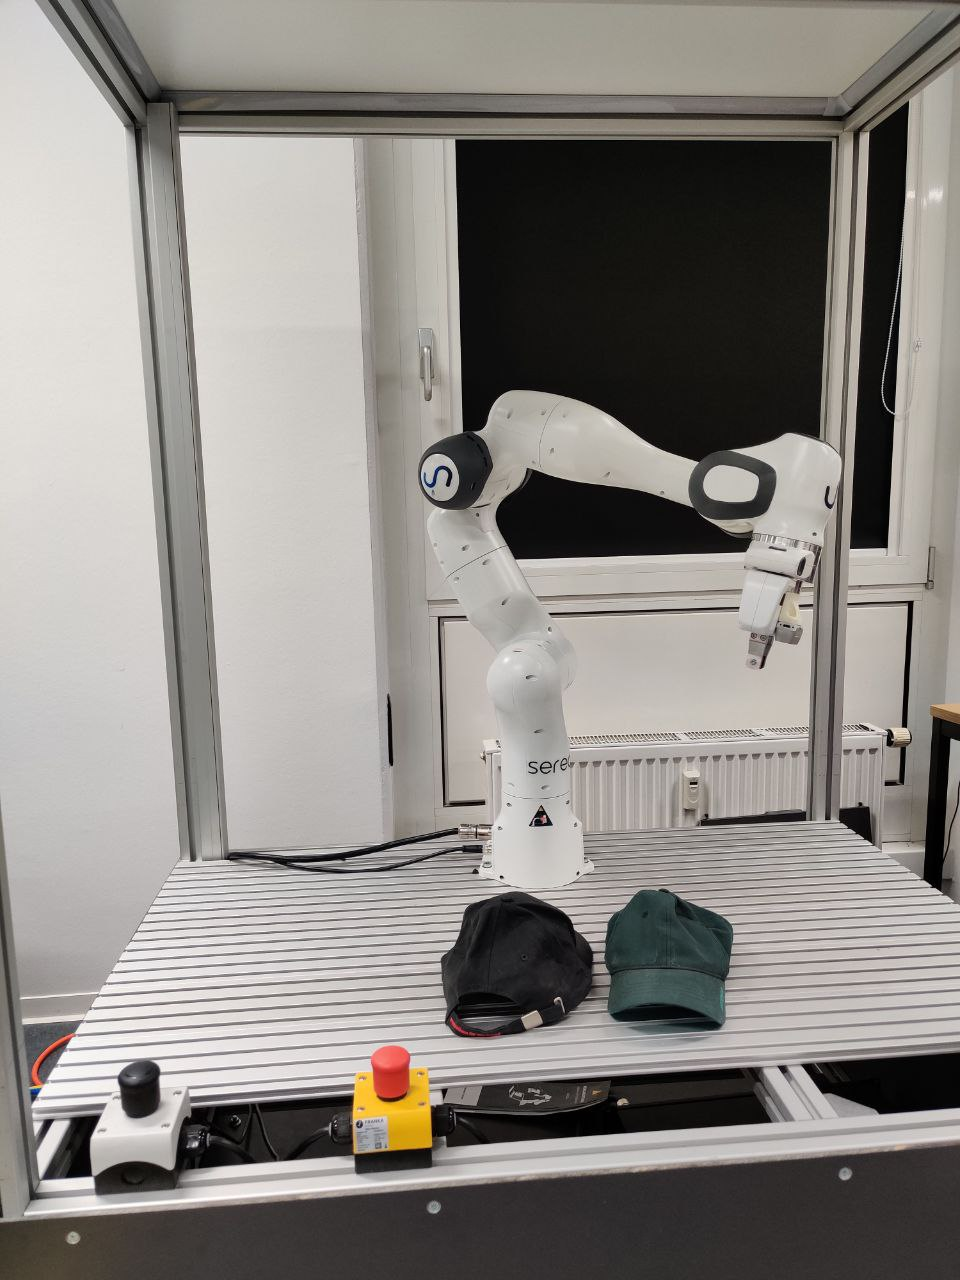
\includegraphics[scale=0.25]{images/robot/setup.jpg}
\end{figure}

The \ac{RGB} image is streamed into the neural networks to compute dense object descriptors from \ac{DON} and 6D pose produced from keypoints from the KeypointNet.
By using pre-computed single class generalized labels stored offline, the Guassian kernel from Equation~\ref{eqn:gaussian_kernel} in page~\pageref{eqn:gaussian_kernel}
is employed to produce grasping points for the robot. The depth information along with camera extrinsic and
intrinsic information is used to project the spatial expectation of the queried label (descriptor) to camera frame coordinate for robot grasping.


\chapter{Results}

\section{Dense Object Nets}

For benchmarking, 48GB VRAM GPU is used. As per the VRAM availability, the \ac{ResNet} architecture with pixelwise distribution and pixelwise nt-xent loss are evaluated
with 2048 correspondences for an image pair with the descriptor dimension $D=3$ and batch size of 2. Additionally, both the loss functions are benchmarked with 512 correspondences
for an image pair with descriptor dimension $D=16$ and batch size of 2. Each model is trained for 100 epochs with Adam optimizer~\cite{kingma2014adam} initialized
with learning rate of $3 \times 10^{-5}$ with weight regularization of $1 \times 10^{-4}$. Minimum validation loss is monitored to save best model.
Each epoch took $45s$. Training \ac{DON} with the pixelwise distribution loss occupies less VRAM compared to the pixelwise nt-xent loss.\\

The $PCK@k$ metric Equation \ref{eqn:pck} is computed following the procedure described in \cite{adrian2022efficient}.
The benchmark results are presented in Table~\ref{table:auc_don}, where the numbers in bold
mark the optimal benchmark result ($\uparrow$ signifies higher score is better). The optimal benchmark result is decided based minimum validation loss and computation costs.\\

The results have higher values compared to benchmarking results in preceeding \cite{adrian2022efficient} as the model is evaluated for a single object scene
rather than for a multi-object scene as described in \cite{adrian2022efficient}. The pixelwise distribution loss outperforms the pixelwise contrastive loss for a single object scene in accordance to the
benchmarks in \cite{adrian2022efficient}.

\begin{table}[htb]
    \centering
    \begin{tabular}{lccccc}
        \hline
        \multicolumn{5}{c}{Benchmarking DON for $AUC \pm \sigma \ for \ PCK@K$ $\uparrow$}                                                                                                                 \\ \hline
        \multicolumn{1}{c}{Loss Functions}         & \multicolumn{1}{c|}{D}  & \multicolumn{1}{c}{\ac{ResNet}-18}      & \multicolumn{1}{c}{\ac{ResNet}-34}      & \multicolumn{1}{c}{\ac{ResNet}-50}      \\ \hline
        \multicolumn{1}{l}{Pixelwise Distribution} & \multicolumn{1}{l|}{3}  & \multicolumn{1}{c}{$\mathbf{0.9800}$}   & \multicolumn{1}{c}{$0.9800$}            & \multicolumn{1}{c}{$0.9800$}            \\
        \multicolumn{1}{l}{Pixelwise Distribution} & \multicolumn{1}{l|}{16} & \multicolumn{1}{c}{$0.9800$}            & \multicolumn{1}{c}{$0.9800$}            & \multicolumn{1}{c}{$0.9800$}            \\
        \multicolumn{1}{l}{Pixelwise NT-Xent}      & \multicolumn{1}{l|}{3}  & \multicolumn{1}{c}{$0.9791 \pm 0.0003$} & \multicolumn{1}{c}{$0.9796 \pm 0.0003$} & \multicolumn{1}{c}{$0.9798 \pm 0.0001$} \\
        \multicolumn{1}{l}{Pixelwise NT-Xent}      & \multicolumn{1}{l|}{16} & \multicolumn{1}{c}{$0.9799 \pm 0.0005$} & \multicolumn{1}{c}{$\mathbf{0.9800}$}   & \multicolumn{1}{c}{$0.9776 \pm 0.0039$} \\ \hline
    \end{tabular}
    \caption{DON evaluation against $AUC \pm \sigma \ for \ PCK@K$ metric.}
    \label{table:auc_don}
\end{table}


\begin{table}[htb]
    \centering
    \begin{tabular}{lc}
        \hline
        \multicolumn{2}{c}{Visual Inspection of Descriptor Image}                                                                                                            \\ \hline
        \multicolumn{1}{c|}{Pixelwise distribution loss }                                         & \multicolumn{1}{c}{Pixelwise NT-Xent loss}                               \\
        \multicolumn{1}{c|}{
\includegraphics[scale=0.2]{images/don/don-d3-resnet50-nc1024-c.png}} & \multicolumn{1}{c}{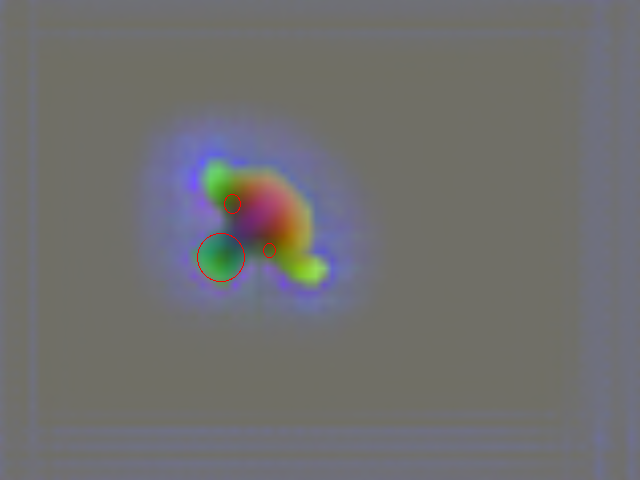
\includegraphics[scale=0.2]{images/don/defects.png} } \\ \hline
    \end{tabular}
    \caption{Visual inspection for optimal placement of descriptors.}
    \label{table:don}
\end{table}

As for the descriptor dimension $D=3$ the pixelwise distribution loss produces consistent results, as described in Table~\ref{table:auc_don}, it is evident that the pixelwise distribution loss produces
optimal descriptors with respect to keypoint spatial expectation compared to the pixelwise nt-xent loss and is chosen for further implementation.\\

To compare both the loss
functions visually, the dense descriptor image is extracted from the \ac{DON} and color encoded by scaling the descriptor ($d \in \mathbb{R}^3$) to the pixel space of $p \in \mathbb{R}^3, \ac{s.t.} \ p \in [0, 255]$. By definition, the dense descriptors are locally
unique to each other. As described in Table~\ref{table:don}, the descriptors encoded by the network trained on the pixelwise nt-xent loss yields the non-optimal descriptors (annotated in red circles in the right image)
compared to the network trained on pixelwise distribution loss which performs better.


\subsection{Manual Method for Robot Grasp Generation}

In the interactive application developed, the descriptors are selected manually. The manually selected descriptors pixels locations are projected to camera frame using depth and camera intrinsics to
produce a 6D pose computed via \ac{PCA}. The \ac{DON} produces consistent descriptors against color jitter, occlusion, illumination and viewpoint detailed in Table~\ref{table:robust_descriptors}. Furthermore, the
6D pose generated via the interactive application is not benchmarked as it is developed to test the consistency of the descriptors produced by \ac{DON} addtionally, the pose produced by \ac{PCA} has different
basis compared to poses present in the dataset.

\begin{table}[htb]
    \centering
    \begin{tabular}{lccccc}
        \hline
        \multicolumn{3}{c}{Illustration of Robust Descriptors}                                                                                                                                                                         \\ \hline
        \multicolumn{1}{c}{Color Jitter}                                       & \multicolumn{1}{c}{Illumination Changes}                               & \multicolumn{1}{c}{Occlusions}                                               \\
        \multicolumn{1}{c}{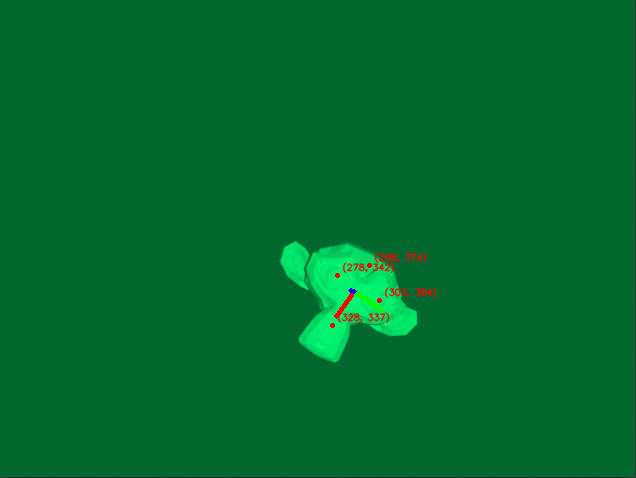
\includegraphics[scale=0.15]{images/don/color.png}} & \multicolumn{1}{c}{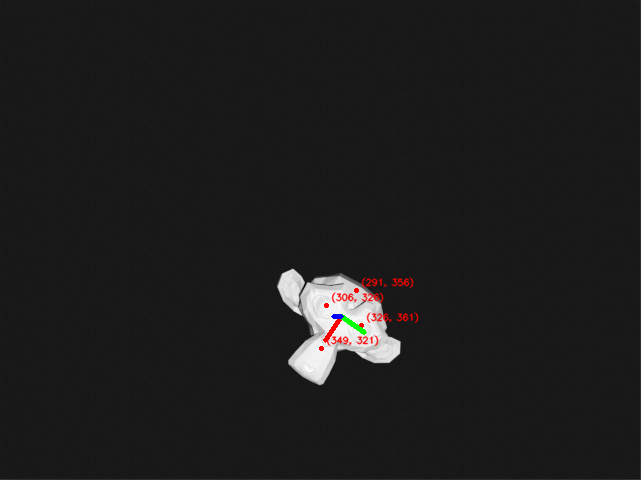
\includegraphics[scale=0.15]{images/don/illum.png}} & \multicolumn{1}{c}{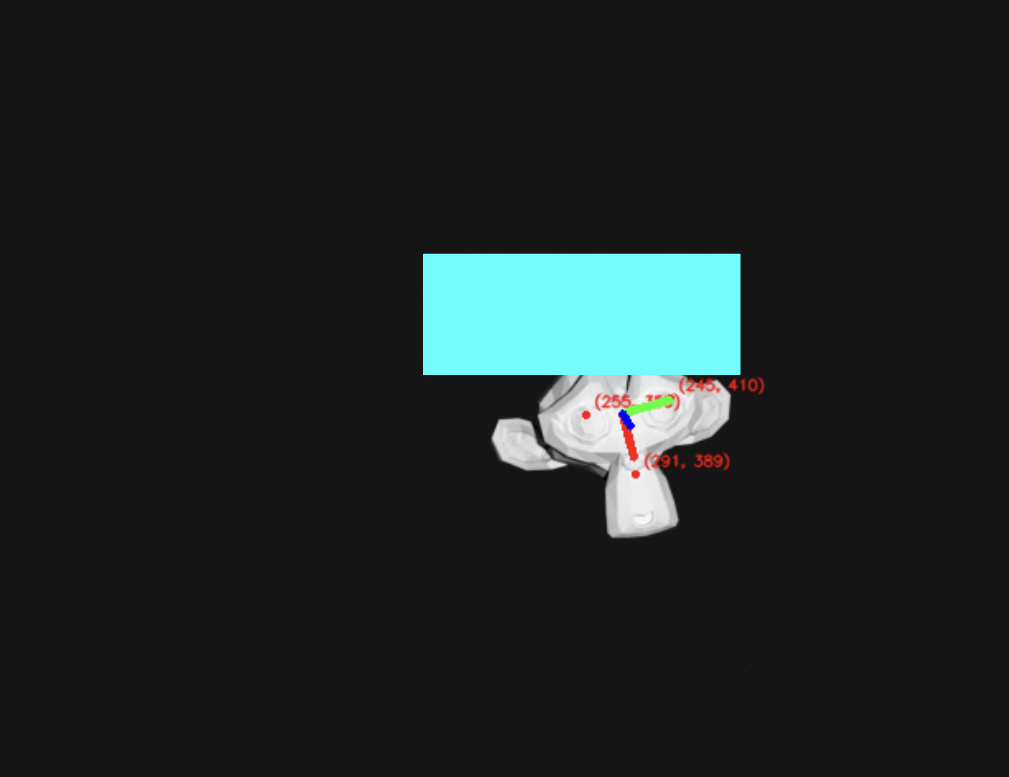
\includegraphics[scale=0.0915]{images/don/occlusion.png}} \\ \hline
    \end{tabular}
    \caption{Testing descriptors for robost 6D pose generation.}
    \label{table:robust_descriptors}
\end{table}








\section{KeypointNet}
\label{subsection:KeypointNet}

The \ac{ResNet} architecture is used to train KeypointNet task for 1000 epochs with batch size 16.
To train the network, ADAM optimizer is used with the learning rate of $1 \times 10^{-3}$ with no weight regularization. The optimal weights to compute
to weighted sum loss in Equation \ref{eqn: weighted_sum} in page \pageref{eqn: weighted_sum} is set to $W=[1.0, 0.2, 1.0, 1.0, 0.0001]^T$. The \ac{ResNet}-18 and \ac{ResNet}-34 architectures are
trained to predict 8, 16, 32 number of geometrically consistent keypoints with $\delta$ = 10 pixel spacing margin. The models are saved monitoring the minimum validation loss while training.\\

To benchmark the KeypointNet, the losses used to train the network itself is applied as it captures information like multiview consistency, relative pose, and whether a keypoint belongs to an object silhoutte, which are the pivotal properties that a keypoint must carry. The Table~\ref{table:keypointnet_benchmark} describes the benchmarking results sampled from 10 random image pairs.
($\downarrow$ in the Table~\ref{table:keypointnet_benchmark} represents that lower score is better.) \\


\begin{table}[htb]
    \centering
    \begin{tabular}{lccccc}
        \hline
        \multicolumn{6}{c}{KeypointNet Benchmarking $\downarrow$}                                                                                                                                                                             \\ \hline
        \multicolumn{1}{c}{Model}          & \multicolumn{1}{c|}{N}  & \multicolumn{1}{c}{$\mathcal{L}_{mc}$}  & \multicolumn{1}{c}{$\mathcal{L}_{pose}$} & \multicolumn{1}{c}{$\mathcal{L}_{obj}$} & \multicolumn{1}{c}{$\mathcal{L}_{sep}$} \\
        \multicolumn{1}{l}{\ac{ResNet}-18} & \multicolumn{1}{l|}{8}  & \multicolumn{1}{c}{$0.1720 \pm 0.0545$} & \multicolumn{1}{c}{$0.0826 \pm 0.1123$}  & \multicolumn{1}{c}{$0 \pm 0$}           & \multicolumn{1}{c}{$0 \pm 0$}           \\
        \multicolumn{1}{l}{\ac{ResNet}-34} & \multicolumn{1}{l|}{8}  & \multicolumn{1}{c}{$0.1115 \pm 0.0244$} & \multicolumn{1}{c}{$0.1303 \pm 0.1325$}  & \multicolumn{1}{c}{$0 \pm 0$}           & \multicolumn{1}{c}{$0.0084 \pm 0.0465$} \\
        \multicolumn{1}{l}{\ac{ResNet}-18} & \multicolumn{1}{l|}{16} & \multicolumn{1}{c}{$0.2121 \pm 0.0676$} & \multicolumn{1}{c}{$0.1427 \pm 0.1332$}  & \multicolumn{1}{c}{$0 \pm 0$}           & \multicolumn{1}{c}{$0.2745 \pm 0.0576$} \\
        \multicolumn{1}{l}{\ac{ResNet}-34} & \multicolumn{1}{l|}{16} & \multicolumn{1}{c}{$0.0830 \pm 0.0891$} & \multicolumn{1}{c}{$0.0732 \pm 0.0891$}  & \multicolumn{1}{c}{$0.1813 \pm 0.2142$} & \multicolumn{1}{c}{$0 \pm 0$}           \\
        \multicolumn{1}{l}{\ac{ResNet}-18} & \multicolumn{1}{l|}{32} & \multicolumn{1}{c}{$1.0130 \pm 0.2978$} & \multicolumn{1}{c}{$0.0990 \pm 0.1276$}  & \multicolumn{1}{c}{$1.3405 \pm 0.3274$} & \multicolumn{1}{c}{$0.0088 \pm 0.0234$} \\
        \multicolumn{1}{l}{\ac{ResNet}-34} & \multicolumn{1}{l|}{32} & \multicolumn{1}{c}{$0.4206 \pm 0.1906$} & \multicolumn{1}{c}{$0.0974 \pm 0.0990$}  & \multicolumn{1}{c}{$0.0928 \pm 0.2440$} & \multicolumn{1}{c}{$0.0122 \pm 0.0508$} \\
        \multicolumn{1}{l}{\ac{ResNet}-50} & \multicolumn{1}{l|}{32} & \multicolumn{1}{c}{$0.1983 \pm 0.6378$} & \multicolumn{1}{c}{$0.1312 \pm 0.1262$}  & \multicolumn{1}{c}{$1.3815 \pm 0$}      & \multicolumn{1}{c}{$0.2019 \pm 0.0829$} \\ \hline
    \end{tabular}
    \caption{Benchmarking KeypointNet with individual losses.}
    \label{table:keypointnet_benchmark}
\end{table}

As per the benchmarking results in Table~\ref{table:keypointnet_benchmark} in page~\pageref{table:keypointnet_benchmark}, the \ac{ResNet}-34 performs better overall.
As per the \ac{ResNet}-18 training history, the validation loss increases after some epochs and does not predict with consistent lower validation loss while, the \ac{ResNet}-34 yields consistent decreasing in
validation loss till the end of the training refer Figure~\ref{fig:output_keypointnet}.  Additionally, \ac{ResNet}-50 is benchmarked to predict 32 keypoints and found under performing. Hence, \ac{ResNet}-34 architecture instead will be used for future implementation.

\begin{figure}[htb]
    \centering
    \caption{Output of trained \ac{ResNet}-34 for KeypointNet task.}
    \label{fig:output_keypointnet}
    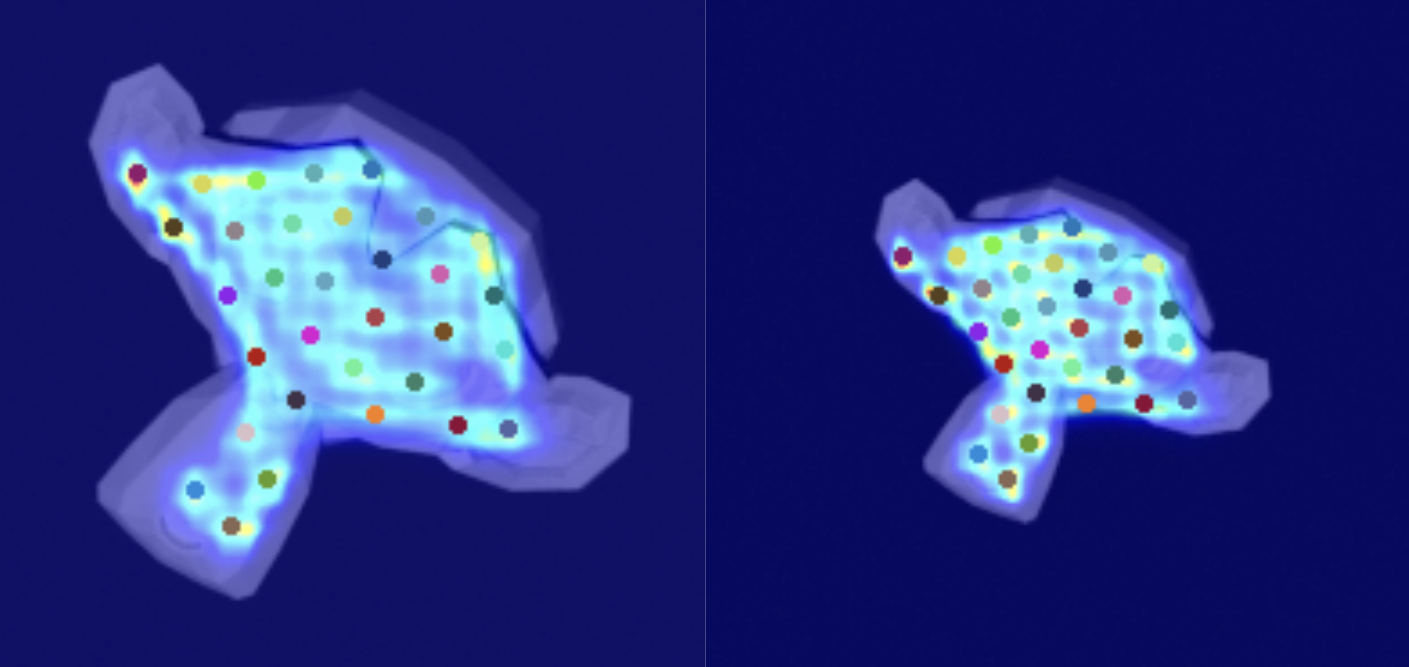
\includegraphics[scale=0.1]{images/keypointnet/output.png}
\end{figure}

\pagebreak





















\section{End-to-End Training}

\subsection{KeypointNet Informed Dense Object Nets}

The \ac{ResNet}-34 is used to implement KeypointNet tasks supplying 256 number of correspondences per image implying 512 correspondences for an image pair to train \ac{ResNet}-18 based \ac{DON} with margin $\delta = 3$ pixel apart.
\ac{DON} is trained with pixelwise distribution loss with the descriptor dimension $D=3$. Adam optimizer is used to train the networks jointly with learning rate of $1 \times 10^{-3}$ and no weight regularization.
$W$ for training the KeypointNet loss is set to the same value as used in KeypointNet benchmarking. The benchmarked results in Table~\ref{table:keypointnet_informed_don_benchmark} in page~\pageref{table:keypointnet_informed_don_benchmark}
are computed by extracting output features from the individual networks stacked to train in end-to-end training fashion.\\

\begin{table}[htb]
    \centering
    \begin{tabular}{lcccc}
        \hline
        \multicolumn{5}{c}{KeypointNet Informed \ac{DON} Benchmarking}                                                                                                                                                              \\ \hline
        \multicolumn{1}{l|}{\ac{DON}}    & \multicolumn{4}{c}{$AUC \pm \sigma \ for \ PCK@K metric$}                                                                                                                                \\
        \multicolumn{1}{l|}{}            & \multicolumn{4}{c}{$0.9666 \pm 0.0034$}                                                                                                                                                  \\ \hline
        \multicolumn{1}{l|}{KeypointNet} & \multicolumn{1}{c}{$\mathcal{L}_{mc}$}                    & \multicolumn{1}{c}{$\mathcal{L}_{pose}$} & \multicolumn{1}{c}{$\mathcal{L}_{obj}$} & \multicolumn{1}{c}{$\mathcal{L}_{sep}$} \\
        \multicolumn{1}{l|}{}            & \multicolumn{1}{c}{$0.4367 \pm 0.9020$}                   & \multicolumn{1}{c}{$0.0893 \pm 0.1897$}  & \multicolumn{1}{c}{$0.0019 \pm 0.0020$} & \multicolumn{1}{c}{$0.0957 \pm 0.0160$} \\ \hline
    \end{tabular}
    \caption{Benchmarking KeypointNet informed \ac{DON} for their individual performance.}
    \label{table:keypointnet_informed_don_benchmark}
\end{table}

The \ac{DON} performance descreases compared to the bechmarking results in Table~\ref{table:auc_don} in page~\pageref{table:auc_don}.
The keypoints computed from the KeypointNet are not consistent as one can see for $ \mathcal{L}_{mc}$ in Table~\ref{table:keypointnet_informed_don_benchmark}.
As the inconsistent keypoints are supplied to \ac{DON} for training, the performance of \ac{DON} decreases. Furthermore, the pixelwise
distribution loss is not robust to inconsistent correspondence as claimed in \cite{florence2020dense}.




























\subsection{Dense Object Nets Informed KeypointNet}

The \ac{ResNet}-18 is used to train \ac{DON} of the descriptor dimension $D=3$ with 256 correspondences per image implying 512 correspondences are sampled to train an image pair.
The \ac{ResNet}-34 is used to train KeypointNet predicting 8 keypoints on dense object representations with $\delta = 10$ pixels apart to pick lables.
ADAM optimizer is used to train the networks jointly with learning rate of $1 \times 10^{-3}$ and no weight regularization.
$W$ for training the KeypointNet loss is set to the same value as used in KeypointNet benchmarking. The benchmarked results in Table~\ref{table:don_informed_informed_benchmark} in page~\pageref{table:don_informed_informed_benchmark}
are computed by extracting output features from the individual networks stacked to train in end-to-end training fashion.

\begin{table}[htb]
    \centering
    \begin{tabular}{lcccc}
        \hline
        \multicolumn{5}{c}{\ac{DON} Informed KeypointNet Benchmarking}                                                                                                                                                              \\ \hline
        \multicolumn{1}{l|}{\ac{DON}}    & \multicolumn{4}{c}{$AUC \pm \sigma \ for \ PCK@K metric$}                                                                                                                                \\
        \multicolumn{1}{l|}{}            & \multicolumn{4}{c}{$0.9756 \pm 0.0005$}                                                                                                                                                  \\ \hline
        \multicolumn{1}{l|}{KeypointNet} & \multicolumn{1}{c}{$\mathcal{L}_{mc}$}                    & \multicolumn{1}{c}{$\mathcal{L}_{pose}$} & \multicolumn{1}{c}{$\mathcal{L}_{obj}$} & \multicolumn{1}{c}{$\mathcal{L}_{sep}$} \\
        \multicolumn{1}{l|}{}            & \multicolumn{1}{c}{$0.4323 \pm 0.1671$}                   & \multicolumn{1}{c}{$0.1048 \pm 0.0476$}  & \multicolumn{1}{c}{$0.0029 \pm 0.0050$} & \multicolumn{1}{c}{$0\pm 0$}            \\ \hline
    \end{tabular}
    \caption{Benchmarking results of \ac{DON} informed KeypointNet with autopicked labels.}
    \label{table:don_informed_informed_benchmark}
\end{table}

As per the benchmarking results in Table~\ref{table:don_informed_informed_benchmark}, the performance of \ac{DON} decreases as the number of correspondences to train the \ac{DON} network is limited to 256 for an image.
This implies that all the loss functions to train the \ac{DON} are sensitive to number of correspondences.\\

The Table~\ref{table:sampled object generalized labels} describes the single class generalized object labels autonomously picked by the KeypointNet from the dense descriptor image. The policy $\pi$ assigns a random
priority to store the labels for `Suzanne' offline. The labels are queried from the descriptor space using 8 keypoints regressed by the KeypointNet with the seperation margin
$\delta = 10$ in pixel space.

\begin{table}[htb]
    \centering
    \begin{tabular}{ll}
        \hline
        \multicolumn{2}{c}{Autosampled single class generalized object label}                     \\ \hline
        \multicolumn{1}{c}{$\pi$(Priority)} & \multicolumn{1}{c}{Label}                           \\ \hline
        \multicolumn{1}{c}{1}               & \multicolumn{1}{c}{$[-3.3778, -3.2668,  6.2417]^T$} \\
        \multicolumn{1}{c}{2}               & \multicolumn{1}{c}{$[-3.4086, -3.3175,  6.2570]^T$} \\
        \multicolumn{1}{c}{3}               & \multicolumn{1}{c}{$[-3.3793, -3.3144,  6.2799]^T$} \\
        \multicolumn{1}{c}{4}               & \multicolumn{1}{c}{$[-3.4003, -3.3314,  6.2663]^T$} \\
        \multicolumn{1}{c}{5}               & \multicolumn{1}{c}{$[-3.3072, -3.1737,  6.1999]^T$} \\
        \multicolumn{1}{c}{6}               & \multicolumn{1}{c}{$[-3.2575, -3.1253,  6.2076]^T$} \\
        \multicolumn{1}{c}{7}               & \multicolumn{1}{c}{$[-3.3644, -3.2777,  6.2714]^T$} \\
        \multicolumn{1}{c}{8}               & \multicolumn{1}{c}{$[-3.3931, -3.2843,  6.2413]^T$} \\ \hline
    \end{tabular}
    \caption{KeypointNet sampled class generalized labels for `Suzanne'.}
    \label{table:sampled object generalized labels}
\end{table}


\subsection{Mining Dense Object Nets Representations in KeypointNet}

The KeypointNet is trained to regress 256 keypoints with $\delta = 2$ using \ac{ResNet}-34 architecture
with the same training setting to benchmark the KeypointNet.
The upsampled dense output feature dimension is reduced to $D=16$ for comparing with the \ac{DON} whose descriptor
dimension is set to $D=16$.\\

The dense representation put forth by the upsampled dense output feature layer is benchmarked against
$PCK@$ as in Equation \ref{eqn:pck} in page~\pageref{eqn:pck}, the same benchmarking process for \ac{DON}.
The upsampled dense output feature evaluates to $AUC \pm \sigma \ for \ PCK@k, \forall k \in [1, 100] = 0.9759 \pm 0.0051$.
This result inlines with the \ac{DON} bechmarked against pixelwise nt-xent loss with descriptor dimension $D = 16$.
Futhermore, the loss for predicting the keypoints increased as illustrated in Figure~\ref{fig:increase_loss_in_keypoints} in page~\pageref{fig:increase_loss_in_keypoints}
as the upsampled dense output feature dimension is reduced from 256 to 16.\\

\begin{figure}[htb]
    \centering
    \caption{Errors in keypoints predictions from KeypointNet modified to benchmark against \ac{DON} representations.}
    \label{fig:increase_loss_in_keypoints}
    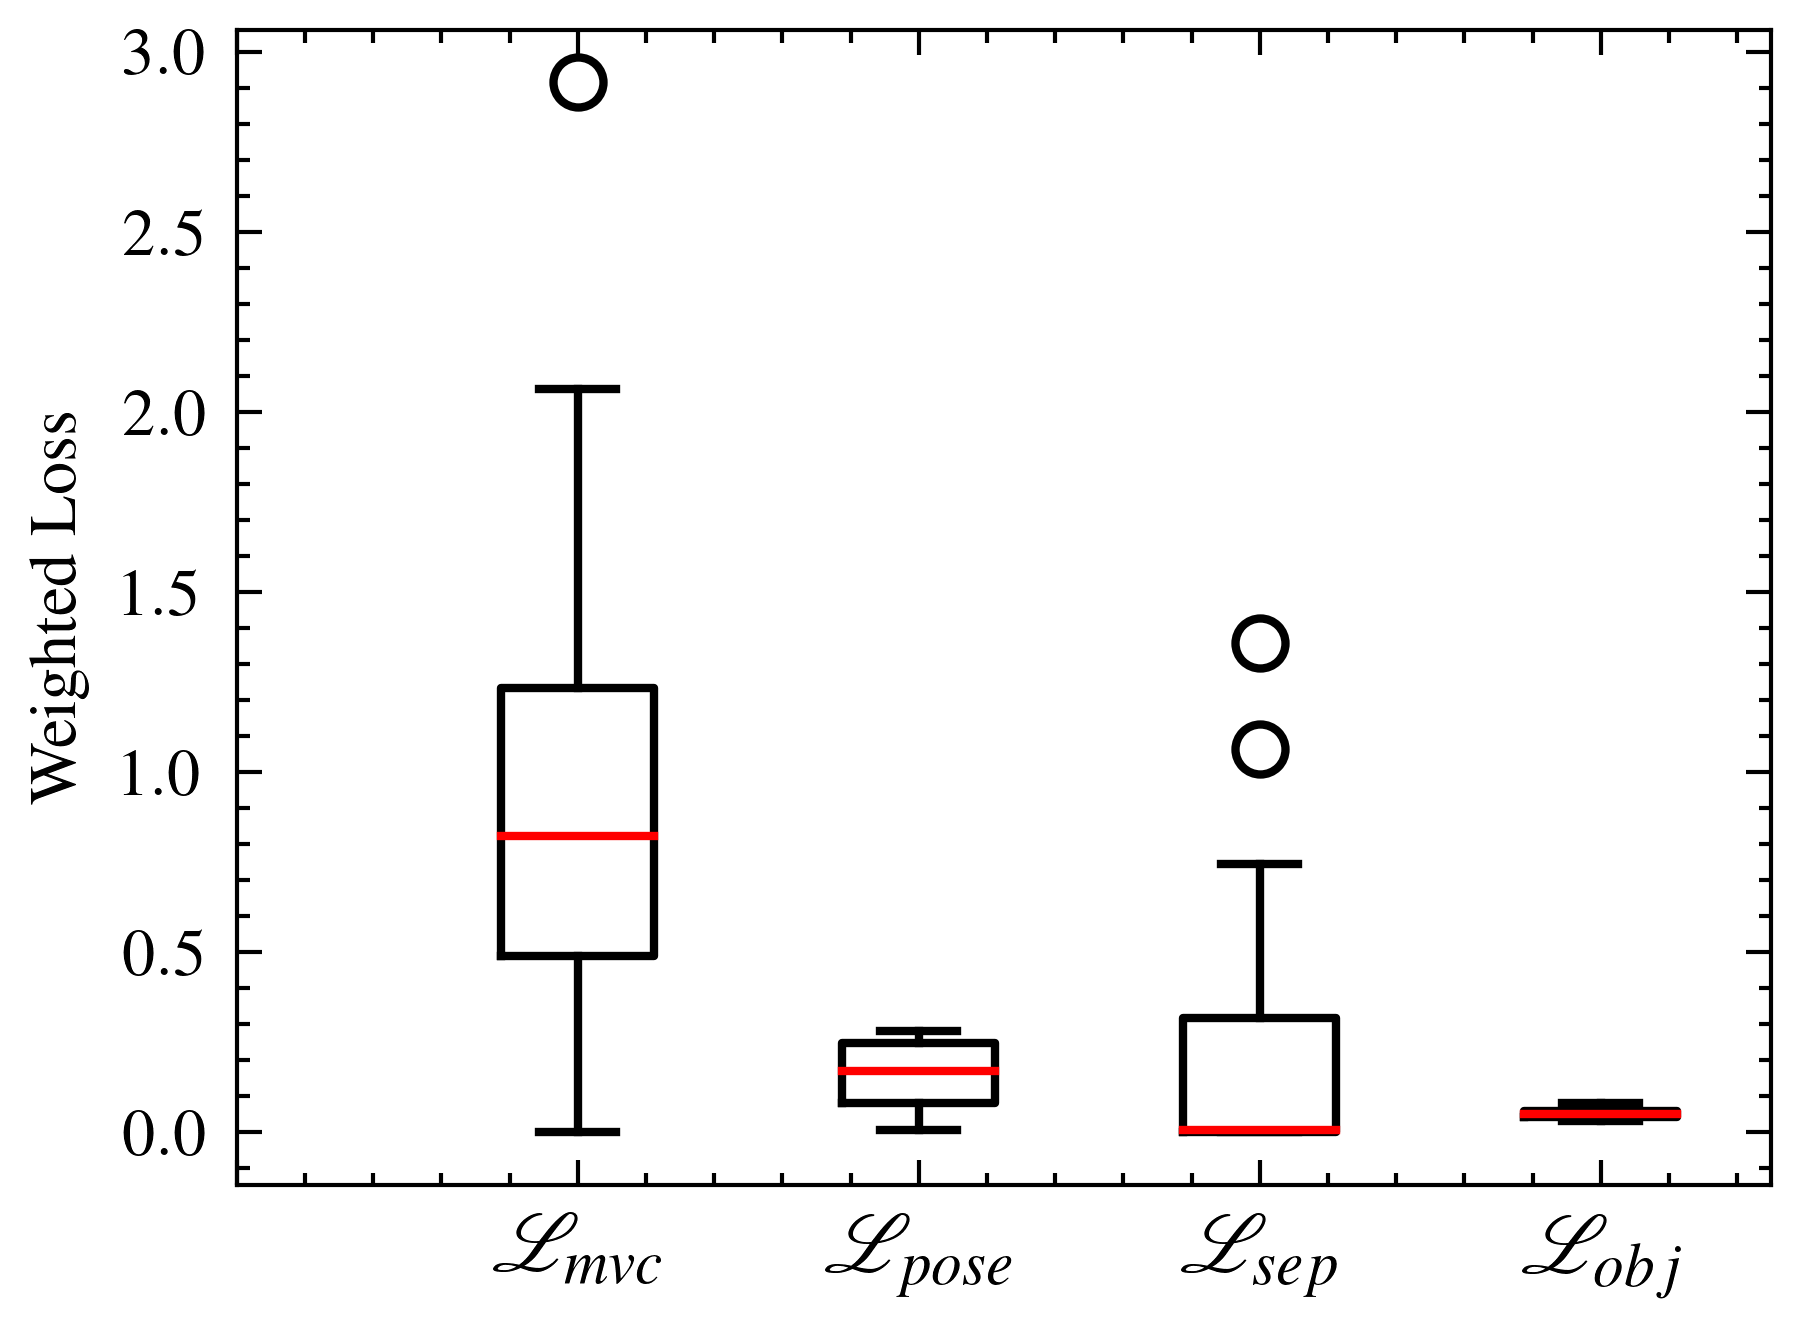
\includegraphics[scale=.75]{images/keypointnet/34-D.png}
\end{figure}


To represent
the descriptor space image of dimension $D = 16$ in an image as in Figure~\ref{fig:descriptors_from_keypointnet}, \ac{PCA} is used to reduce
the dimension to a higher dimensional sub-space of $D = 3$ (a higher dimensional sub-space is the lower dimensional representation of a higher dimension).
\ac{PCA} is only used for visualization purposes. The representation is not consistent as \ac{PCA} preserves variance in the data while
projecting it to a higher dimensional sub-space explaining the ears of `Suzanne' with same color.
No further attempts are carried out to represent dense descriptor images in an image as it does not align with the thesis objective.

\begin{figure}[htb]
    \centering
    \caption{Depiction of dense descriptors extracted from KeypointNet.}
    \label{fig:descriptors_from_keypointnet}
    
\includegraphics[scale=0.22]{images/don/don-d16-resnet50-nc256-c.png}
\end{figure}





















































\section{Generalizing ``Caps''}

\subsection{Semantic Correspondence Mapping Pipeline}

KeypointNet is trained to predict $100$ keypoints with pixel spacing margin $\delta = 5$. Adam optimizer is used to train
the network for 1000 epochs with a learning rate $1 \times 10^{-3}$ and no weight regularization. The $W$ is set similarly to the same value as in the KeypointNet benchmarking. Furthermore, Keypointnet is based on \ac{ResNet}-34 architecture with upsampled dense output dimension set to $256$.\\

The KeypointNet is benchmarked for its loss function as detailed in  Table~\ref{table:benchmark_semantic_correspondence} in page~\pageref{table:benchmark_semantic_correspondence}. The benchmarking yields higher errors
compared to the results in Table~\ref{table:keypointnet_benchmark} in page~\pageref{table:keypointnet_benchmark} as the number of correspondences is higher and semantically equivalent objects are trained. For the visual inspection purposes, $8$  keypoints are sampled randomly as in the Table~\ref{table:visual_inspection_semantic_correspondence}
in page~\pageref{table:visual_inspection_semantic_correspondence}. Most of the keypoints are semantically well placed, with a few keypoints regressed with high multiview consistent errors.\\


\begin{table}[htb]
    \centering
    \begin{tabular}{lcccc}
        \hline
        \multicolumn{4}{c}{Semantic Correspondence Mapping Pipeline Benchmarking}                                                                                              \\
        \multicolumn{1}{c}{$\mathcal{L}_{mc}$}  & \multicolumn{1}{c}{$\mathcal{L}_{pose}$} & \multicolumn{1}{c}{$\mathcal{L}_{obj}$} & \multicolumn{1}{c}{$\mathcal{L}_{sep}$} \\ \hline
        \multicolumn{1}{c}{$5.1342 \pm 2.8517$} & \multicolumn{1}{c}{$0.1456 \pm 0.0628$}  & \multicolumn{1}{c}{$0.2135 \pm 0.0771$} & \multicolumn{1}{c}{$2.0256 \pm 1.2637$} \\ \hline
    \end{tabular}
    \caption{Benchmarking: KeypointNet used for mapping semantic correspondences.}
    \label{table:benchmark_semantic_correspondence}
\end{table}


\begin{table}[htb]
    \centering
    \begin{tabular}{lcccc}
        \hline
        \multicolumn{3}{c}{Visual Inspection of Semantic Correspondences}                                                                                                                                                           \\ \hline
        \multicolumn{1}{c}{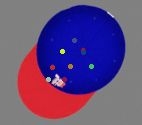
\includegraphics[scale=0.87]{images/cap/image_a.png}} & \multicolumn{1}{c}{\includegraphics[scale=1]{images/cap/image_b.png}} & \multicolumn{1}{c}{
\includegraphics[scale=0.95]{images/cap/image_c.png}} \\ \hline
    \end{tabular}
    \caption{Illustration of semantic correspondences. The semantic correspondences are color coded.}
    \label{table:visual_inspection_semantic_correspondence}
\end{table}

Furthermore, the semantic correspondence pipeline is examined for the root cause of the high errors.
The semantic correspondence pipeline did not converge for a cap in the synthetic dataset.
As illustrated in Figure~\ref{fig:non_convergence} in page~\pageref{fig:non_convergence}, the keypoints do not meet
the properties of geometrically consistent keypoints further, explaining the high errors in Table~\ref{table:benchmark_semantic_correspondence}
in page~\pageref{table:benchmark_semantic_correspondence}. The object is removed from the dataset, and the
semantic correspondence pipeline is trained again to resolve predictions of keypoints with errors.
The errors decrease after another training as seen in Table ~\ref{table:revised_benchmark_semantic_correspondence} in page~\pageref{table:revised_benchmark_semantic_correspondence}.

\begin{figure}[htb]
    \centering
    \caption{Non-Convergence in Semantic Correspondence Pipeline.}
    \label{fig:non_convergence}
    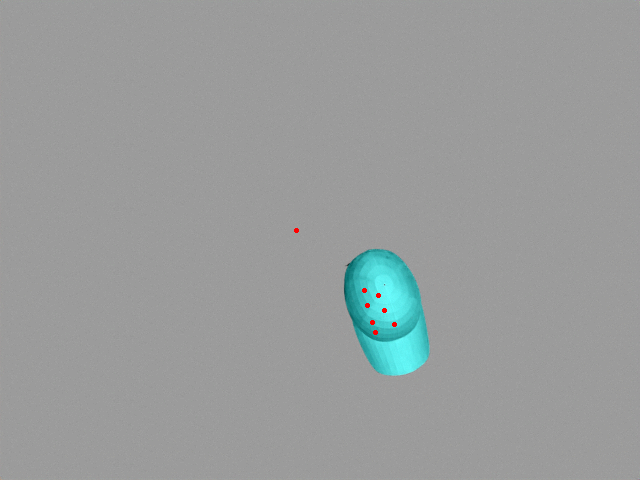
\includegraphics[scale=0.2]{images/cap/defect_a.png}
\end{figure}

\begin{table}[htb]
    \centering
    \begin{tabular}{lcccc}
        \hline
        \multicolumn{4}{c}{Revised Semantic Correspondence Mapping Pipeline Benchmarking}                                                                                      \\ \hline
        \multicolumn{1}{c}{$\mathcal{L}_{mc}$}  & \multicolumn{1}{c}{$\mathcal{L}_{pose}$} & \multicolumn{1}{c}{$\mathcal{L}_{obj}$} & \multicolumn{1}{c}{$\mathcal{L}_{sep}$} \\ \hline
        \multicolumn{1}{c}{$2.1210 \pm 1.5937$} & \multicolumn{1}{c}{$0.0754 \pm 0.1840$}  & \multicolumn{1}{c}{$0.0780 \pm 0.0079$} & \multicolumn{1}{c}{$0.1374 \pm 1.8752$} \\ \hline
    \end{tabular}
    \caption{Revised bechmarking for semantic correspondences mapping pipeline.}
    \label{table:revised_benchmark_semantic_correspondence}
\end{table}


\subsection{Evaluating Single Class Generalized Labels in the Wild}

Two images of caps were collected using a smartphone with a camera to benchmark single-label generalizing ability in the wild as illustrated in Table~\ref{table:cap_wild} in page~\pageref{table:cap_wild}.
Furthermore, from now on, benchmarking method initially used to quantify the neural network tasks will not be used.\\

\begin{table}[htb]
    \centering
    \begin{tabular}{lcccc}
        \hline
        \multicolumn{2}{c}{Caps in the Facility}                                                                                                        \\
        \multicolumn{1}{c}{
\includegraphics[scale=0.1]{images/cap/wild_a.jpg}} & \multicolumn{1}{c}{
\includegraphics[scale=0.1]{images/cap/wild_b.jpg}} \\ \hline
    \end{tabular}
    \caption{Depiction of two caps found in the facility.}
    \label{table:cap_wild}
\end{table}

For evaluating \ac{DON} trained on the synthetic dataset of caps, \ac{DON} is trained with \ac{ResNet}-34 architecture with pixelwise correspondence loss with the dense
descriptor dimension $D=3$ as it is previously found to be performing optimally as can be seen in Table~\ref{table:auc_don} in page \pageref{table:auc_don} and computationally economical.
Additionally, \ac{DON} is trained on the semantic correspondences supplied from the KeypointNet, and ADAM optimizer is used with a learning rate of $3 \times 10^{-5}$
with weight regularization set to $1 \times 10^{-4}$ for 100 epochs with batch size 2.\\

The trained \ac{DON} is tested on the cap images. Judging from
Figure~\ref{fig:caps_in_wild_testing}, the descriptors are not placed semantically well. The heatmaps in the image describe a descriptor's spatial probability in two images. The heatmaps are generated from the interactive
application developed to generate robot grasps manually with the temperature parameter set to $t=-0.3$ in Gaussian kernel search space Equation \ref{eqn:gaussian_kernel} in
page~\pageref{eqn:gaussian_kernel}.\\

\begin{figure}[htb]
    \centering
    \caption{Testing optimal descriptor placement for the caps in the wild.}
    \label{fig:caps_in_wild_testing}
    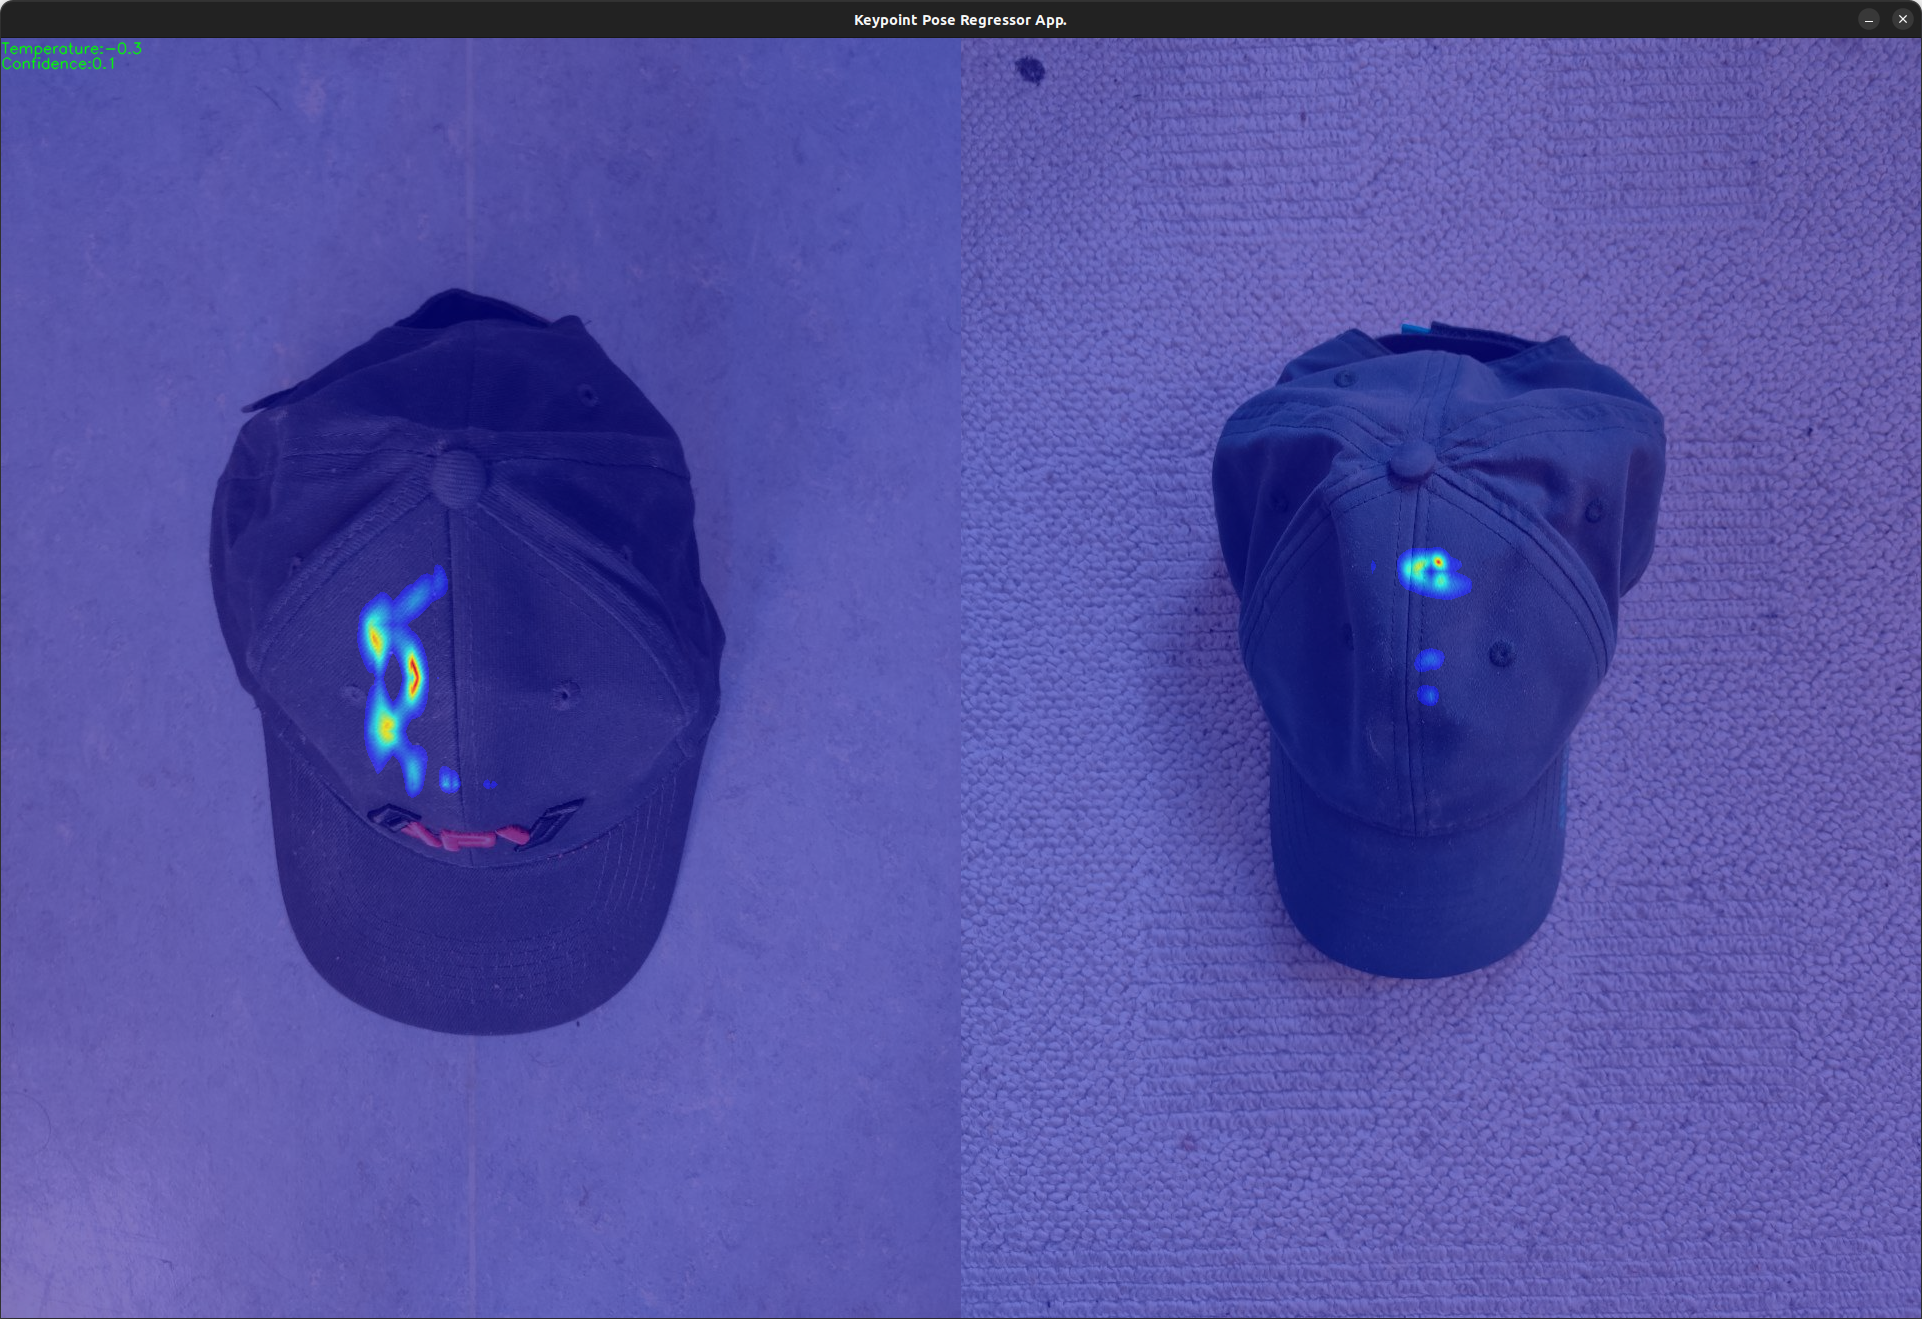
\includegraphics[scale=0.1]{images/cap/heatmaps.png}
\end{figure}

Furthermore, the \ac{DON} is testing using interactive application on the synthetic dataset.
As illustrated in the Figure~\ref{fig:don_performing_optimally} in page~\pageref{fig:don_performing_optimally}, the \ac{DON} performs optimally. The \ac{DON} places spatially optimal descriptors semantically across the objects in the same class.\\

\begin{figure}[htb]
    \centering
    \caption{\ac{DON} performing optimally on the synthetic dataset}
    \label{fig:don_performing_optimally}
    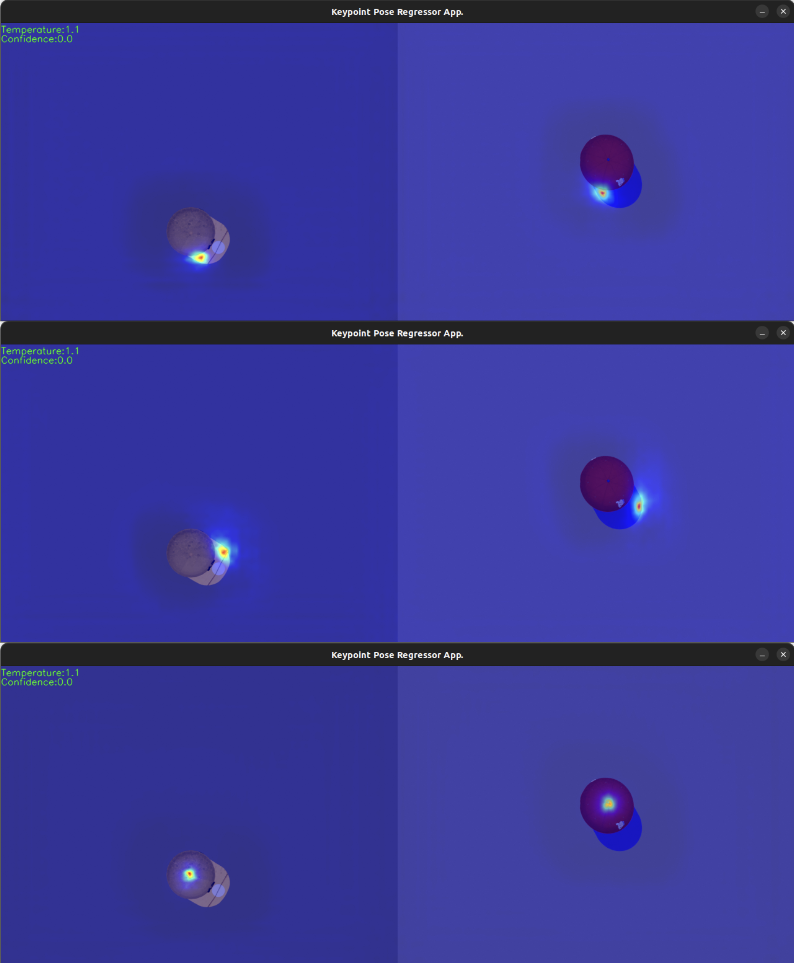
\includegraphics[scale=0.25]{images/cap/heatmaps_dataset.png}
\end{figure}

The synthetic dataset is perfect without any faults compared to the real-world data. Despite using background randomizations, noisy backgrounds, colour jitters and greyscaling augmentations, the \ac{DON} performs poorly on the real-world data as the
descriptors are not placed spatially optimally in the semantically same objects.

\subsection{\emph{``Not losing hope on the real world''}}

As per the results, the neural networks perform optimally locally in synthetic data and not real data, further posing an issue for robot grasping.\\

The neural network implementation scheme has three parts i.e., semantic correspondence mapping pipeline, \ac{DON} and KeypointNet to pick auto labels.
As the semantic correspondence pipeline is noisy and converged with errors as highlighted in Table~\ref{table:revised_benchmark_semantic_correspondence} in page~\pageref{table:revised_benchmark_semantic_correspondence},
the method of generating synthetic correspondences are adopted from \cite{adrian2022efficient} to train \ac{DON}. Furthermore, the \ac{DON} informed KeypointNet is adapted to regress
three keypoints on \ac{DON} representations generating geometrically consistent 6D poses.\\

To compute synthetic correspondences, the spatial grid $\mathcal{G}$ as in Equation \ref{eqn:spatial_grid} in page~\pageref{eqn:spatial_grid} is stacked
with the \ac{RGB} image such that the image dimension is as follows:

\begin{equation}
    I \rightarrow \mathbb{R}^{H \times W \times \mathbf{5}}
\end{equation}

Furthermore, the image is affinely augmented with previously used augmentations from the vision library provided by \cite{paszke2019pytorch}. Correspondences are the intersection of the spatial grid in the augmented image and the anchor image as illustrated in the Figure~\ref{fig:synthetic_correspondences}
in page~\pageref{fig:synthetic_correspondences}. These synthetic correspondences are further consumed to train \ac{DON}.

\begin{figure}[htb]
    \centering
    \caption{Illustrations of synthetic correspondences computed from the image augmentation. The pixel annotated in blue in the left image corresponds to the same pixel annotated in green in the right image.}
    \label{fig:synthetic_correspondences}
    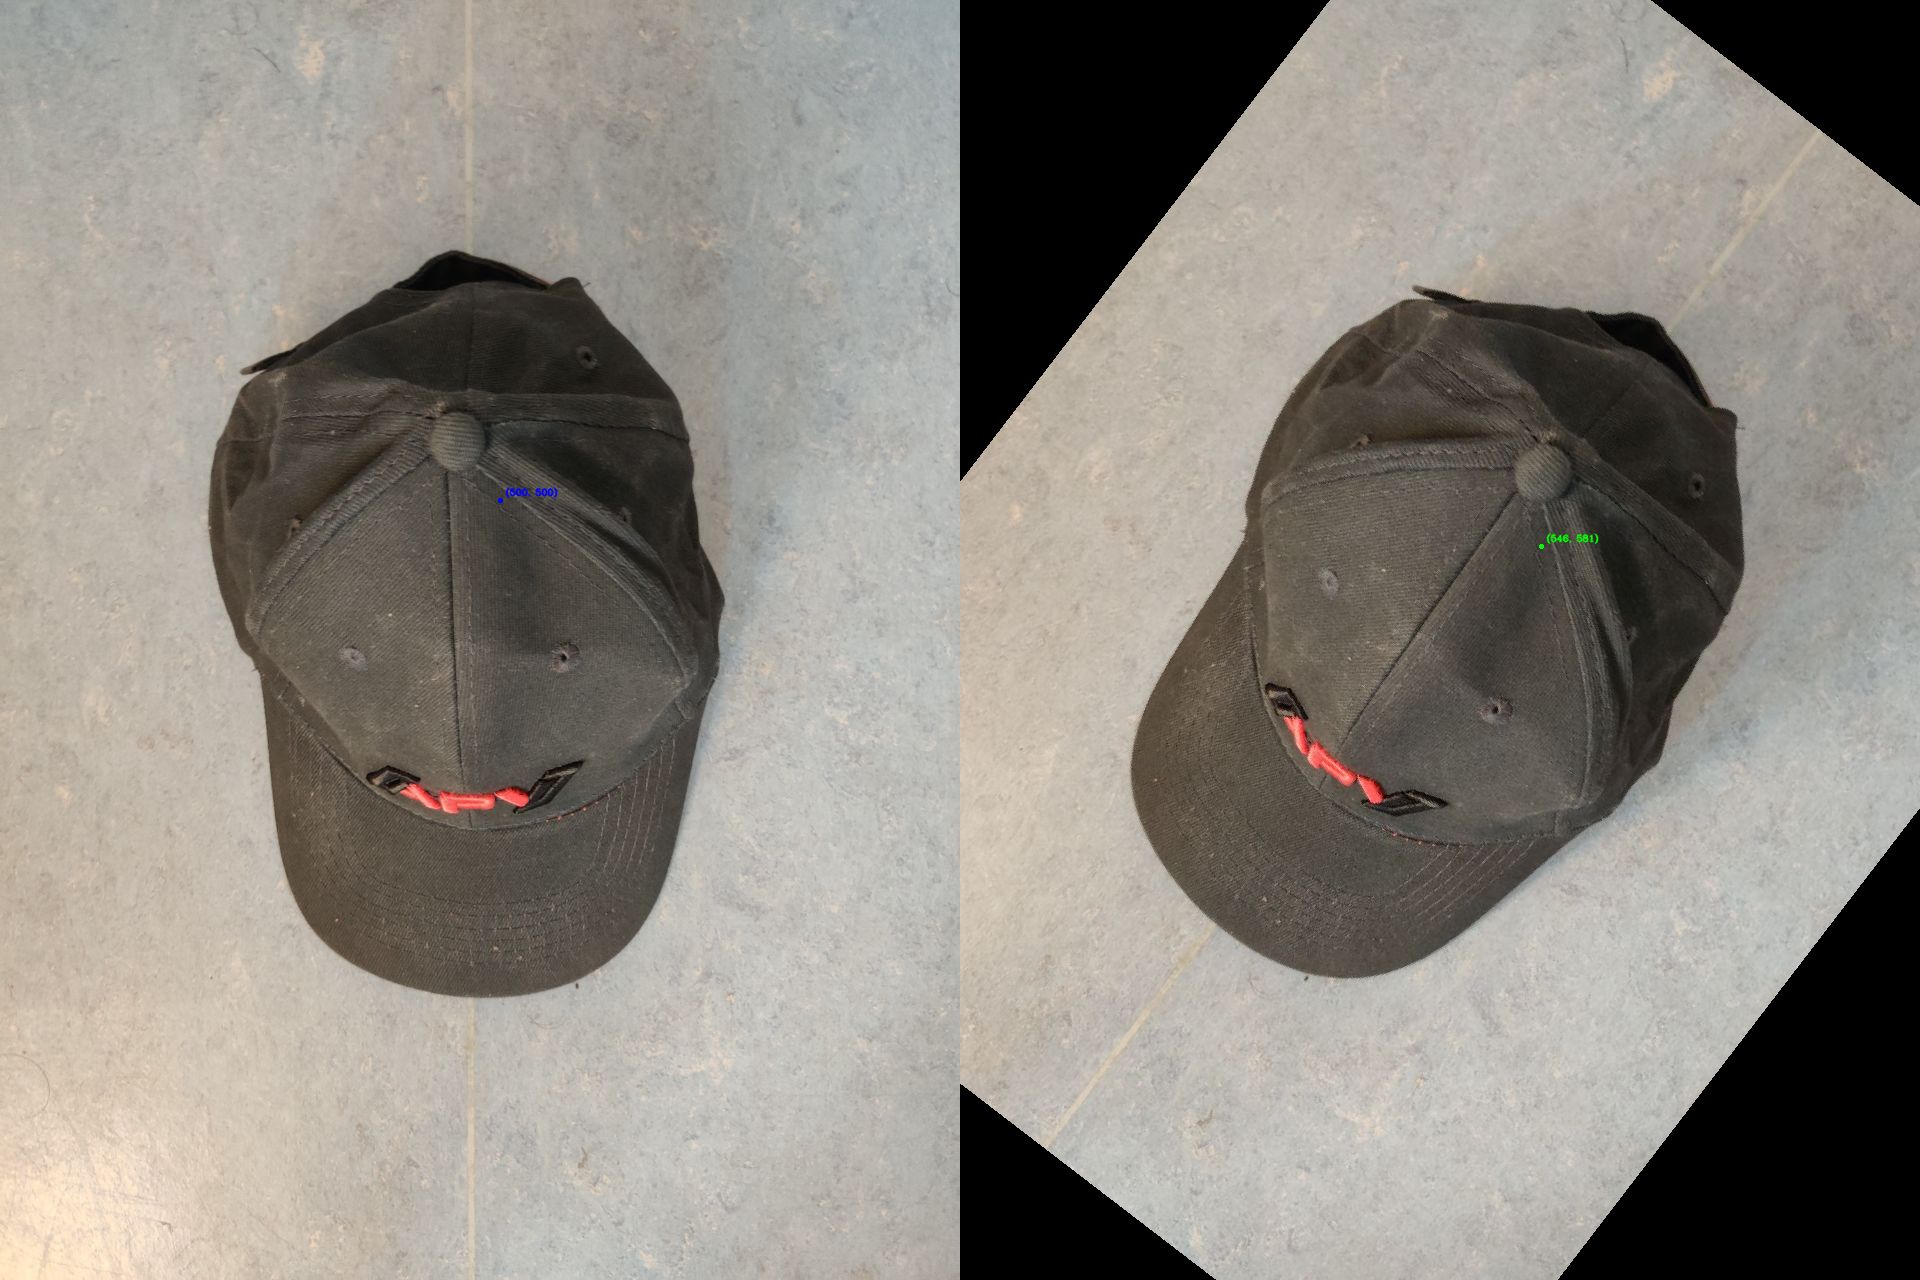
\includegraphics[scale=0.1]{images/cap/aug_image.png}
\end{figure}

The synthetic correspondences generalize caps in the real world pretty well, as depicted in the Figure~\ref{fig:real_heatmaps} in page~\ref{fig:real_heatmaps}.

\begin{figure}[htb]
    \centering
    \caption{Visual inspection of \ac{DON} trained on synthetic correspondences.}
    \label{fig:real_heatmaps}
    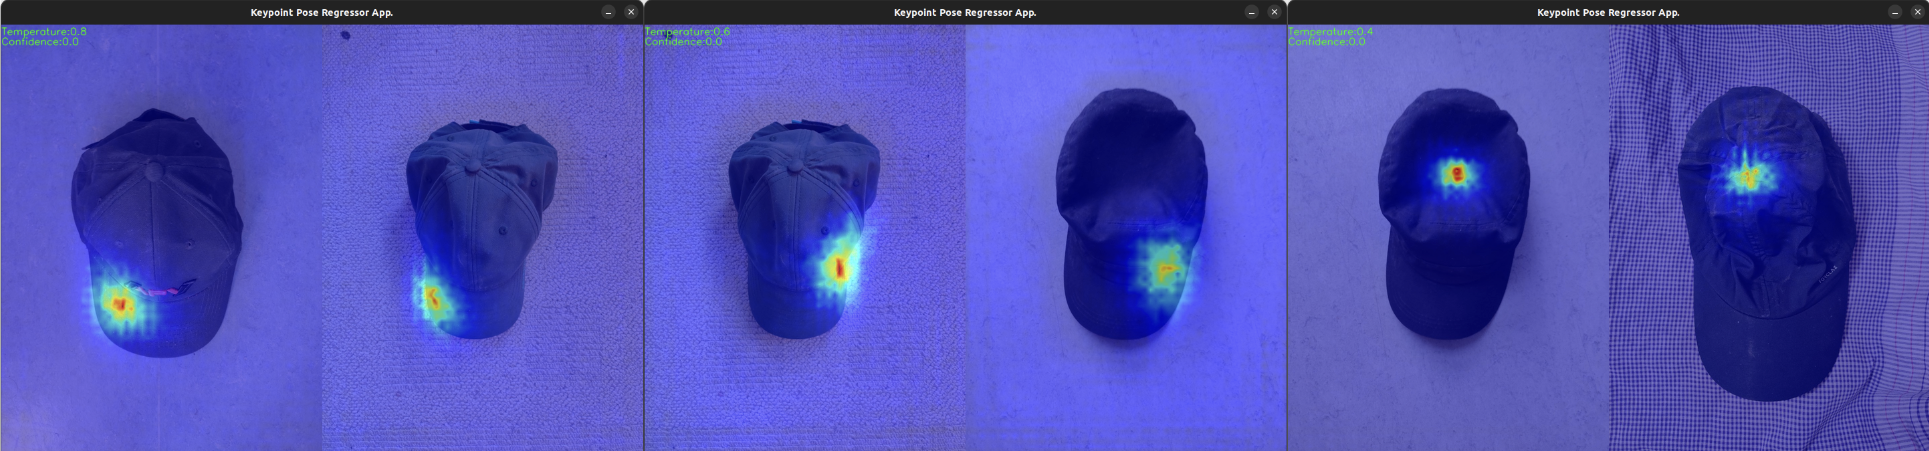
\includegraphics[scale=0.2]{images/cap/real_heatmap.png}
\end{figure}


\subsection{Robot Grasping Pipeline}

The KeypointNet is trained on the \ac{DON} representations to regress 3 geometrically consistent keypoints on dense descriptor images. These keypoint locations are the location of the dense descriptor labels.
Furthermore, these labels are stored offline in the .json format as rendered in the Listing~\ref{lst:json} in page~\pageref{lst:json}
for querying the descriptors in the real-time application.

\begin{lstlisting}[language=json, firstnumber=1, caption=Preview of json file entry of offline stored descriptors., label={lst:json}]
    ["cap":{
            "labels":[
                [3.1030, -3.4000, 2.9119],
                [5.2890, -2.5363, -0.7921],
                [0.0596, -3.8049, 2.1469]
            ]
            "priority":[
                1,
                2,
                3
            ]
        }
    ]
\end{lstlisting}

Both \ac{DON} and \ac{DON} informed KeypointNet, networks compute robot grasping poses as described below.

\subsubsection{Straight 3D Grasps with \ac{DON}}

As illustrated in Figure~\ref{fig:straight_grasp} in page~\pageref{fig:straight_grasp}, the robot moves to a position to capture the image of the cap. The \ac{RGB} image is fed into the \ac{DON} to compute a dense descriptor image.
The labels previously stored in .json format are read and extracted based on the priority to produce spatial expectation in the descriptor space.
The depth map is further used to project the spatial expectation and depth to camera coordinates for generating straight robot grasps.

\begin{figure}[htb]
    \centering
    \caption{3D grasping pipeline.}
    \label{fig:straight_grasp}
    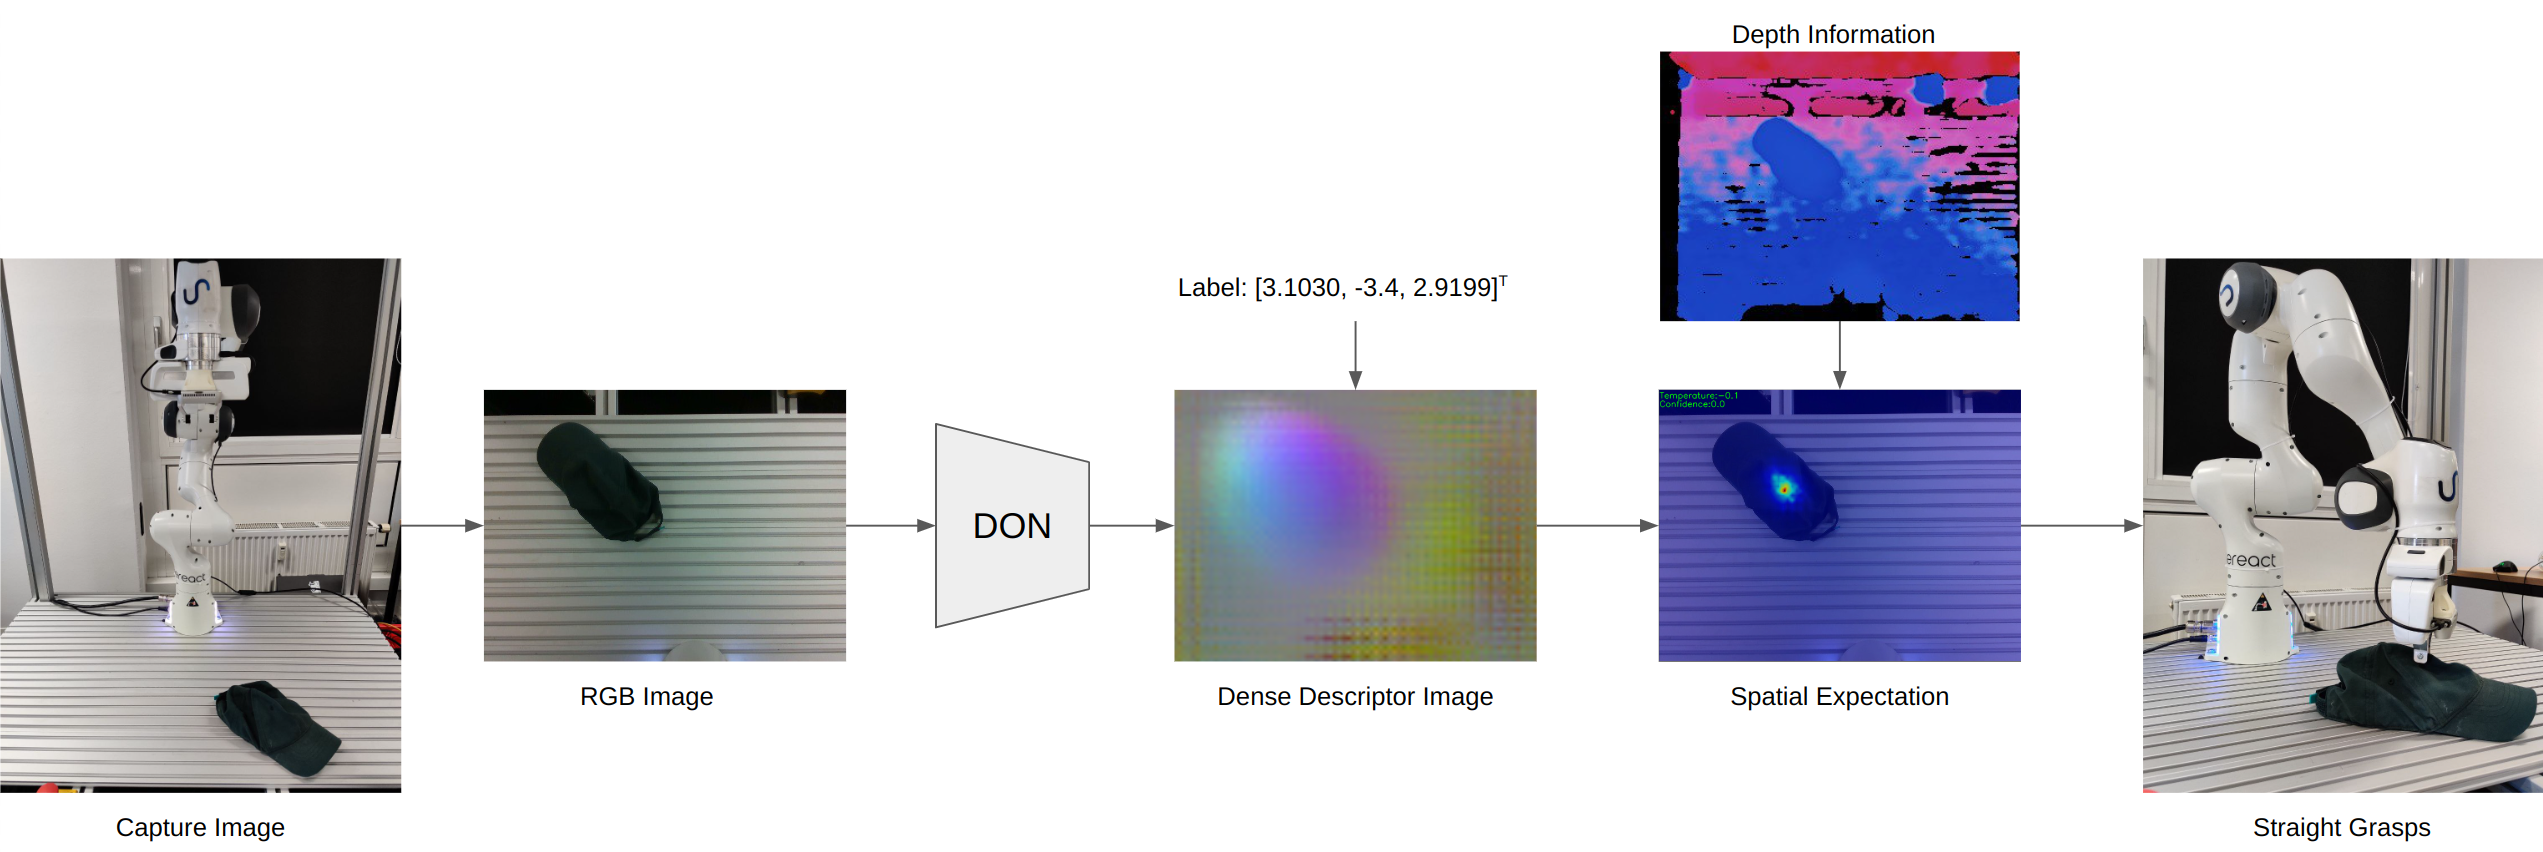
\includegraphics[scale=0.15]{images/robot/straight_grasps.png}
\end{figure}


\subsubsection{Aligned 6D Grasps with \ac{DON} Informed KeypointNet}

As depicted in Figure~\ref{fig:aligned_grasps}, the robot moves to a position to capture the image of the cap. The \ac{RGB} image is fed into the \ac{DON} Informed KeypointNet to compute object 6D pose. The robot
realigns the gripper according to the computed object 6D pose and, grasps the object.

\begin{figure}[htb]
    \centering
    \caption{6D grasping pipeline.}
    \label{fig:aligned_grasps}
    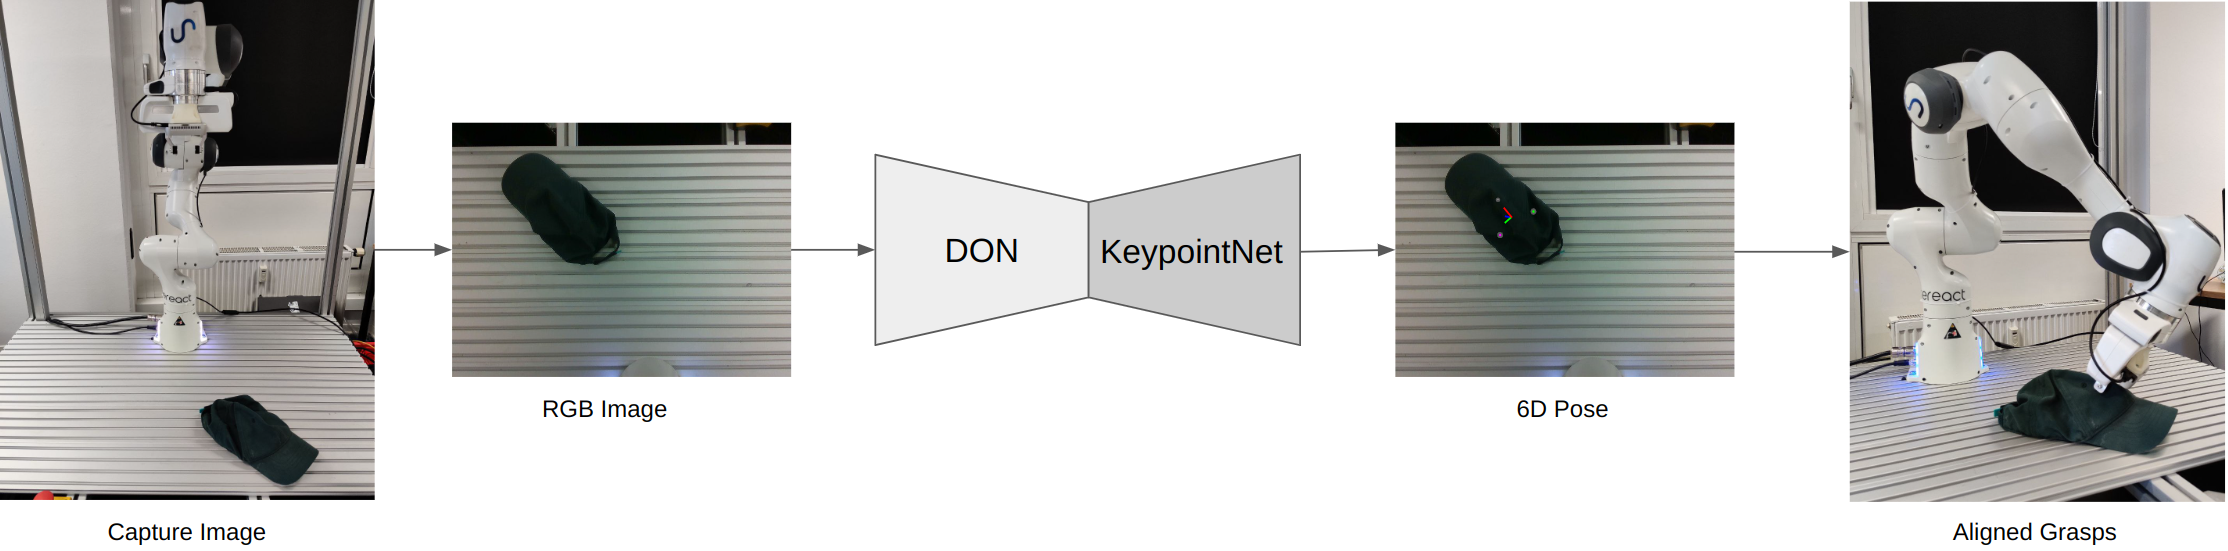
\includegraphics[scale=0.15]{images/robot/aligned.png}
\end{figure}

\subsubsection{Autonomous Robot Grasping Routine}

Figure~\ref{fig:complete_pipeline} depicts the autonomous robot grasping pipeline.
The robot consistently picks the cap robustly using both methods of generating grasps and places the caps aligned, mimicking the industrial robot palletizing routine effectively.

\begin{figure}[htb]
    \centering
    \caption{Autonomous robot grasping routine.}
    \label{fig:complete_pipeline}
    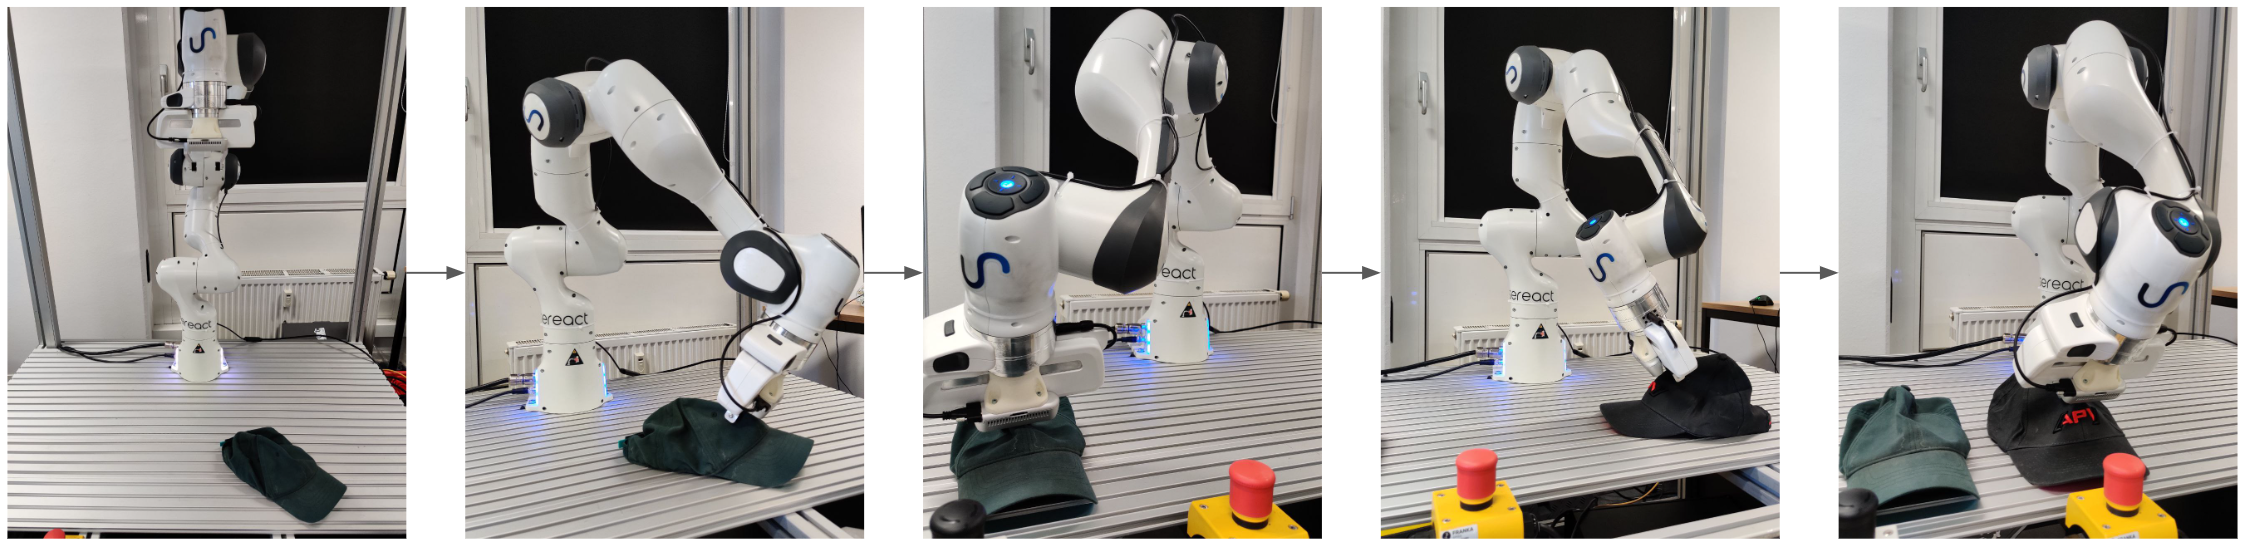
\includegraphics[scale=0.15]{images/robot/cycle.png}
\end{figure}
\chapter{Conclusion}

The thesis set off with the aim of creating artificial intelligence for robots like Chappie and C-3PO.
These robots can perform generalized tasks rather than task-oriented activities, which is the present state of today's artificial intelligence.
In particular, the thesis focused on developing generalized representations of an object in an image for robot manipulation solving the present industrial robotics
problem of teaching robots to pick every object equipped with 2D or 3D vision systems eliminating the need for explicit programming for each object.\\

Set on to implement artificial intelligence with generalizing capabilities, \ac{DON} is implemented.
The \ac{DON} is introduced to the robotics community by  \citeauthor{florence2018dense}~\cite{florence2018dense} with generalization capabilities of objects in an image.
The \ac{DON} generates dense descriptor image from an \ac{RGB} image capable of generalizing an object for robot manipulation.
Furthermore, the thesis benchmarked various loss functions, different \ac{ResNet}
neural networks. We have identified that, the ``Pixelwise Distribution Loss'' with \ac{ResNet}-34 performs best to generalize objects belonging to the same class (i.e., semantically equivalent) and moreover is computationally
economical compared to ``Pixelwise NT-Xent Loss''.
Single class generalized labels manually extracted from the pixels of the dense descriptor image provided by \ac{DON} are applied to various applications like generating robust object 6D poses of objects in cases of illumination changes,
colour changes, occlusion and different viewpoints and other application being robot grasping.\\

To eliminate the need of manually selecting labels from the dense descriptor image put forth by the \ac{DON}, KeypointNet is implemented.
The KeypointNet, as described, predicts a set of oriented geometrically consistent keypoints on an object such that it preserves the object's 6D pose.\\

The KeypointNet comes with generalizing properties as it predicts geometrically consistent keypoints across objects belonging to the same class. The generalizing property
of KeypointNet is exploited to create a semantic correspondence pipeline to train the \ac{DON}, replacing the need for depth information which is often noisy with today's technology of depth cameras available.
Additionally, the KeypointNet is trained on manifold-based loss making it faster to converge and the need of an orientation network is eliminated.
Furthermore, the manifold loss implemented to train the KeypointNet limits the object rotation to a range of $[0, \pi]$. The \ac{ResNet}-34 architecture performs optimally for the predicting geometrically consistent keypoints.
The KeypointNet is sensitive to occlusion and fails to predict keypoints on occluded areas of objects encountered in the training phase. \\


As \ac{DON} is robust against occlusion, KeypointNet could benefit from it. KeypointNet trained on \ac{DON} representations, regresses a keypoint that occupies a pixel in the dense descriptor image later where
this pixel location is queried as a single class generalized label eliminating any need for
human intervention.\\

The upsampled dense output put forth by the KeypointNet represents dense object representations as an alternative to \ac{DON} to create single-class
generalized labels. This ushers an idea that there are other networks capable of computing
dense descriptors image similarly to \ac{DON}.\\


Initially, the networks are trained on synthetic data. The synthetic data is too perfect to be generalized on real-world objects. The KeypointNet and \ac{DON} trained
on the synthetic dataset did not perform well in the wild. The end-to-end training of neural networks showed reduced performance when trained with the synthetic dataset.\\

Synthetic correspondences introduced in \cite{adrian2022efficient} are used to overcome the limitations of training the networks posed by the synthetic data.
The synthetic correspondences are independent of camera intrinsic and extrinsic information, including depth information to compute correspondences.
The \ac{DON} is trained on images of caps captured from a smartphone with a camera with synthetic correspondence and performed well, generalizing most of the caps in the wild.\\

The capabilities of \ac{DON} and KeypointNet are demonstrated and applied to generalized autonomous robot task of cap pick-and-place operation.
\chapter{Future Scope}
As the Keypointnet is limited by the manifold losses for training objects with rotation in range $[0, \pi]$, a newer formulation will be engineered and applied.
Furthermore, KeypointNet and \ac{DON} will be expanded to accommodate objects belonging to different classes.\\

As of this writing, the \ac{DON} training cannot accommodate multiple similar object in an image as it is limited by the presented loss functions \parencites{florence2020dense}{adrian2022efficient}.
To overcome this, ``Ranked InfoNCE Loss'' \cite{hoffmann2022ranking} will be adopted on the pixelwise scale to train \ac{DON} accommodating multiple similar
objects in a scene.\\

To build up appropriate states for the future robot path planning and grasping using model-based reinforcement learning \cite{kaiser2019model},
\ac{DON} computed dense descriptor image will be encoded to a vector
state $x \in \mathbb{R}^D$ instead of $I_D \in \mathbb{R}^{H \times W \times D}$ with the neural networks inspired from \cite{tschannen2018recent} for faster online training.
The robot path planning will be based on the KeypointNet alternatively to the method trajectory generation proposed in \parencites{florence2019self}.


%\chapter{Conclusions}

% ********************************************************************
% End of contents
% ********************************************************************

\cleardoublepage
\printbibliography

\cleardoublepage
\addchap{List of Acronyms} % Abkürzungsverzeichnis


\begin{acronym}[ResNet]
    \acro{RGB}{3-Channel Image}
    \acro{RGB-D}{4-Dimensional Image, i.e., RGB with Depth}
    \acro{CNN}{Convolutional Neural Network}
    \acro{DL}{Deep Learning}
    \acro{DNN}{Deep Neural Network}
    \acro{DON}{Dense Object Nets}
    \acro{ISW}{Institut für Steuerungstechnik der Werkzeugmaschinen und Fertigungseinrichtungen \acroextra{der Universität Stuttgart}}
    \acro{NeRF}{Neural Radiance Fields}
    \acro{NDA}{Non-Disclosure Agreement}
    \acro{PCA}{Principal Component Analysis}
    \acro{ResNet}{Residual Network}
    \acro{s.t.}{such that}
    \acro{SIFT}{Scale-Invariant Feature Transform}
    \acro{SVD}{Singular Value Decomposition}
    \acro{SOTA}{State of the Art}
    \acro{SPS}{Speicherprogrammierbare Steuerung}
    \acrodefplural{SPS}[SPS]{Speicherprogrammierbare Steuerungen}
\end{acronym}

\cleardoublepage
\listoffigures

\cleardoublepage
\listoftables
\lstlistoflistings

\cleardoublepage
\addchap{List of Symbols}




\begin{longtable}{@{}l p{10cm}@{}}
    \toprule
    Symbol                              & Description                               \\
    \midrule
    \endfirsthead
    \multicolumn{2}{c}{\textit{List of Symbols -- continued}}                       \\
    \toprule
    Symbol                              & Description                               \\
    \midrule
    \endhead
    \bottomrule \multicolumn{2}{r}{\textit{Continued on next page}}                 \\
    \endfoot
    \bottomrule
    \endlastfoot

    % start here with your symbols:
    \(\mathbf{D}\)                      & Dense descriptor dimension                \\
    \(\mathbb{N}^+\)                    & Set of positive integers                  \\
    \(\in\)                             & Belongs to or in                          \\
    \(\mathcal{M} \)                    & Riemannian manifold                       \\
    \(SO\left(n\right)\)                & Special orthogonal group of dimension $n$ \\
    \(SE\left(3\right)\)                & Special euclidean group of dimension 3    \\
    \(\mathbb{R}^n\)                    & Real number of dimension $n$              \\
    \(\left< \cdot \ ,\ \cdot \right>\) & Scalar product of two vectors             \\
    \(\| \ \cdot \ \|\)                 & $L^2$ Norm                                \\
    \(\| \ \cdot \ \|_F\)               & Frobenius Norm                            \\
\end{longtable}

%% Appendix, if needed:
% \appendix
% \chapter{Example appendix chapter}

\end{document}